%versi 2 (8-10-2016)\chapter{Landasan Teori}
\label{chap:teori}
\section{Privasi}
Privasi adalah adalah kemampuan satu atau sekelompok individu untuk menutupi atau melindungi kehidupan dan urusan personalnya dari publik dengan mengontrol sumber-sumber informasi mengenai diri mereka. Sebelum melindungi privasi sebuah data, diperlukan pemahaman untuk membedakan jenis atribut yang bersifat sensitif dan non-sensitif. 

\par Personally Identifiable Information  (PII) adalah standar yang digunakan untuk menentukan apakah informasi yang ada dapat melakukan identifikasi entitas individu secara lansung atau tidak langsung. PII menjelaskan bahwa identifikasi entitas secara langsung dapat dilakukan menggunakan atribut sensitif. Sedangkan identifikasi entitas secara tidak langsung dapat dilakukan menggunakan penggabungan beberapa atribut non-sensitif. 
\\\\
Berikut adalah contoh informasi yang bersifat sensitif menurut standar PII:

\begin{itemize}
\item Identitas diri seperti nama lengkap, tempat tanggal lahir, alamat rumah, alamat email.
\item Nomor identitas diri seperti NIK, nomor passport, nomor SIM, nomor wajib pajak, nomor rekening, nomor telepon, dan nomor kartu kredit.
\item Karakteristik pribadi seperti foto diri, sidik jari, dan tulisan tangan.
\item Data biometrik seperti pemindaian retina, jenis suara, dan geometri wajah.
\item Aset informasi lainnya seperti IP Address dan Media Access Control (MAC). 
\end{itemize}

\noindent Berikut adalah contoh informasi yang bersifat non-sensitif menurut standar PII:
\begin{itemize}
\item Rekaman medis
\item Riwayat pendidikan
\item Riwayat pekerjaan 
\item Informasi finasial
\item Letak geografis
\end{itemize}


\par Untuk melakukan publikasi data dari satu perusahaan ke perusahaan lain digunakan teknik anonimisasi untuk melindungi dan menyamarkan atribut sensitif pada masing-masing data, sehingga data yang diterima oleh perusahaan lain tidak dapat dilakukan identifikasi. Sebagai contoh, perusahaan asuransi ingin membagikan informasi dengan perusahaan pemasaran. Maka perusahaan ansuransi akan menyamarkan data yang bersifat sensitif dan menyediakan data terkait dengan kebutuhan perusahaan pemasaran. 


\newpage
\section{Data Mining}
Data yang dikumpulkan oleh sistem informasi semakin bertambah banyak. Oleh karena itu, perlu adanya cara untuk melakukan proses ekstraksi informasi pada sekumpulan data yang sangat banyak. Menurut Gartner, data mining adalah proses menemukan korelasi, pola, dan tren baru yang bermakna dengan menyaring sejumlah besar data yang disimpan menggunakan teknologi pengenalan pola serta teknik statistik dan matematika. Data mining merupakan bagian dari Knowledge Discovery in Databases (KDD). KDD adalah proses transformasi sekumpulan data yang disimpan pada basis data menjadi informasi yang berguna.\\

\begin{figure}[H]
	\centering
	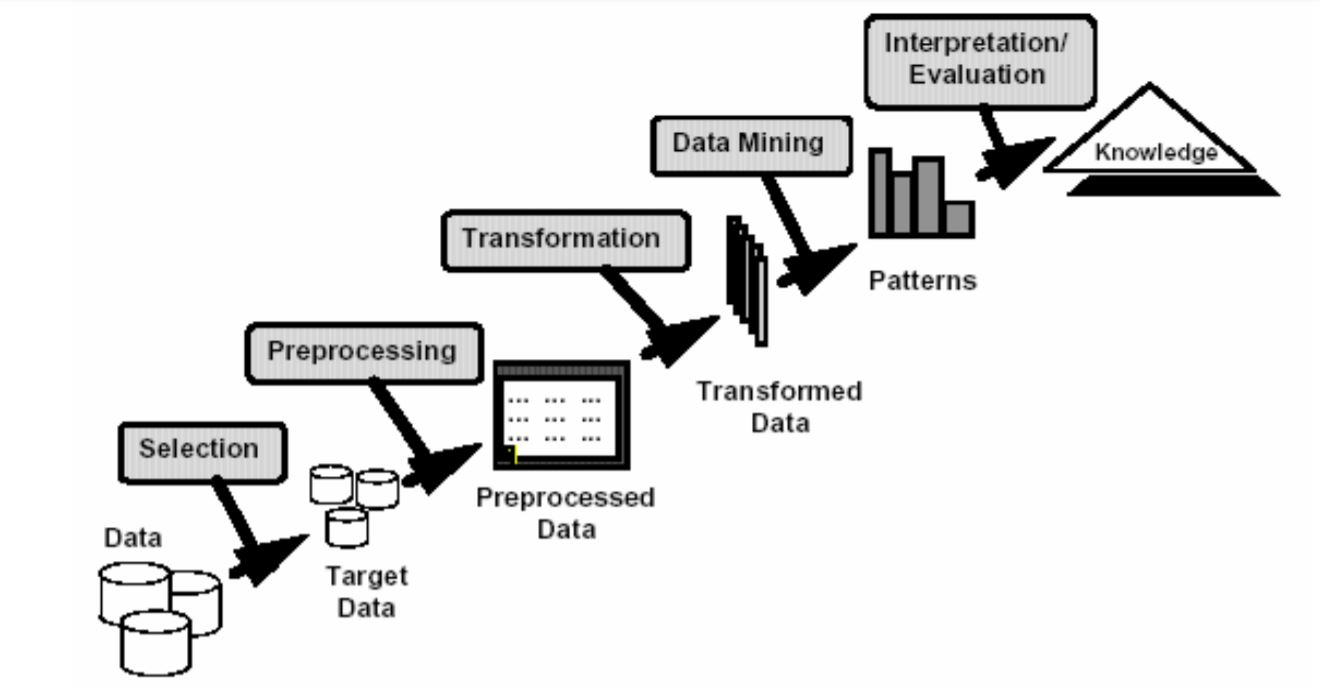
\includegraphics[scale=0.3]{datamining1}
	\caption{Tahapan pada KDD}
	\label{fig:datamining1}
\end{figure}

\noindent Berikut ini adalah penjelasan tahapan pada KDD pada Gambar \ref{fig:datamining1} sebagai berikut:

\begin{enumerate}
\item Selection adalah proses mengambil data yang relevan terhadap analisis.
\item Preprocessing adalah proses pembersihan data dengan menghilangkan data yang tidak konsisten dan integrasi data dengan menggabungkan beberapa data dari sumber yang berbeda.
\item Transformation adalah proses manipulasi data menggunakan konsep agregasi, generalisasi, normalisasi, dan reduksi agar data tersebut dapat dipakai sesuai kebutuhan analisis.
\item Data Mining adalah proses ekstraksi informasi dari sekumpulan data yang telah diolah pada tahap sebelumnya, menggunakan metode yang umum digunakan untuk mengenali pola seperti klasifikasi, pengelompokan/clustering.
\item Interpretation/Evaluation adalah proses interpretasi hasil pengolahan data menjadi sebuah grafik yang dapat dimengerti, sehingga dapat disimpulkan menjadi sebuah pengetahuan.
\end{enumerate}

\noindent Tantangan yang sering muncul pada penggunaan teknik data mining adalah sebagai berikut:

\begin{itemize}
\item Skalabilitas, artinya data yang ingin diolah berukuran sangat besar.
\item Dimensionalitas yang tinggi, artinya data memiliki jumlah jenis atribut yang sangat banyak.
\item Data yang heterogen, artinya munculnya jenis data terstruktur, semi-terstruktur, dan tidak struktur.
\end{itemize}

\noindent Tujuan dari penggunaan teknik data mining adalah sebagai berikut:

\begin{itemize}
\item Prediksi adalah menggunakan nilai dari beberapa atribut yang sudah ada untuk memprediksi nilai atribut di masa yang akan datang, contohnya adalah klasifikasi.
\item Deskripsi adalah menemukan pola-pola yang dapat merepresentasikan kelompok dari sebuah data, contohnya adalah pengelompokan/clustering.
\end{itemize}

\section{Klasifikasi} 
Klasifikasi adalah proses menemukan model (atau fungsi) yang cocok untuk mendeskripsikan dan membedakan sebuah kelas data dengan kelas data lain. Dalam pembelajaran mesin, klasifikasi sering dianggap sebagai contoh dari metode pembelajaran yang diawasi, yaitu menyimpulkan fungsi dari data pelatihan berlabel. Tugas klasifikasi adalah  menganalisis data pelatihan dan menghasilkan fungsi yang tepat untuk digunakan dalam menentukan kelas dari data baru  dengan menetapkan label kelas yang benar untuk masing-masing data. Metode klasifikasi memerlukan  analisis relevansi antar atribut untuk mengidentifikasi atribut yang akan dipakai pada proses klasifikasi. Atribut tersebut dipilih sebelum proses klasifikasi dimulai. Atribut lain yang tidak relevan terhadap proses klasifikasi dapat diabaikan. 
\\
\begin{figure}[H]
	\centering
	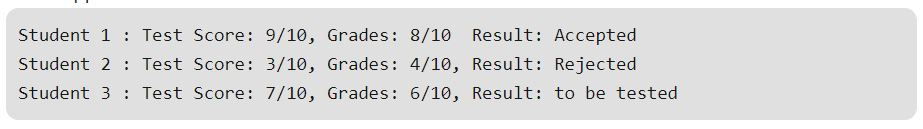
\includegraphics[scale=0.45]{klasifikasi1}
	\caption{Jenis Pemodelan Klasifikasi}
	\label{fig:klasifikasi1}
\end{figure}

\noindent Pada Gambar \ref{fig:klasifikasi1}, klasifikasi dapat dimodelkan dengan 3 cara yaitu (a) IF-THEN, (b) Decision Tree, dan (c) Neural Network. Setiap model memiliki caranya masing-masing untuk melakukan proses klasifikasi pada data pelatihan. Algoritma klasifikasi biasanya  menggunakan salah satu model dari ketiga jenis pemodelan tersebut. Berikut adalah penjelasan singkat dari ketiga jenis pemodelan klasifikasi  pada Gambar \ref{fig:klasifikasi1} yang umum digunakan: 

\begin{itemize}
\item IF-THEN adalah pemodelan klasifikasi data dengan diberikan kondisi-kondisi tertentu yang bersifat unik  untuk merepresentasikan hasil dari klasifikasi kelas.
\item Decision Tree adalah pemodelan klasifikasi data dengan menggunakan analogi struktur pohon, di mana setiap cabang mewakili jenis nilai atribut pada sebuah node dan setiap daun mewakili hasil dari klasifikasi kelas.
\item Neural Network adalah pemodelan klasifikasi data menggunakan analogi neuron pada jaringan syaraf, di mana neuron adalah node yang saling terhubung dan memiliki bobot antar node untuk klasifikasi kelas.
\end{itemize}

\newpage
\section{Naive bayes}
\par Naive bayes menerapkan metode klasifikasi probabilistik. Jenis klasifikasi ini menghasilkan probabilitas yang sesuai untuk masing-masing kelas yang mungkin. Kelas dengan probabilitas tertinggi akan dipilih sebagai kelas terbaik. Naive bayes menggunakan teorema bayes. Naive bayes mengasumsikan bahwa fitur tertentu tidak selalu berhubungan dengan fitur lainnya. Naive bayes mudah untuk dibangun dan memiliki komputasi yang lebih cepat daripada model klasifikasi lainnya untuk dataset berukuran sangat besar. 
\\\\
\noindent Kelebihan dari Naive bayes adalah sebagai berikut:

\begin{itemize}
\item Memiliki kinerja yang cepat untuk melakukan klasifikasi data.
\item Membutuhkan data pelatihan yang lebih sedikit dibandingkan model lain.
\item Implementasi lebih mudah dibandingkan model lain.
\end{itemize}

\noindent Kekurangan dari Naive bayes adalah sebagai berikut:

\begin{itemize}
\item Tidak dapat membuat prediksi untuk probabilitas yang bernilai nol.
\item Hanya bergantung pada nilai probabilitas saja sehingga hasil prediksi menjadi kurang baik.
\end{itemize}
 
\noindent Teorema Bayes dapat dinyatakan dalam rumus sebagai berikut:

\begin{equation}
P(H|D) = \frac{P(D|H) \cdot P(H)}{P(D)}
\end{equation}

\noindent Probabilitas hipotesis tertinggi dapat dinyatakan dalam rumus sebagai berikut:

\begin{align}
MAP(H) = max(P(H|D))
\end{align}

\noindent Keterangan:
\begin{itemize}
\item P(H|D) adalah probabilitas posterior apabila diberika hipotesis H dan diketahui data D. 
\item P(D|H) adalah probabilitas posterior  data d jika hipotesis h adalah benar.
\item P(H) adalah probabilitas hipotesis h adalah benar 
\item P(D) adalah probabilitas data.
\end{itemize}

\noindent Secara singkat, langkah kerja algoritma Naive Bayes dapat dijelaskan sebagai berikut:

\begin{enumerate}
\item Menghitung probabilitas masing-masing kelas.\\
Probabilitas kelas dapat dihitung berdasarkan f data dari masing-masing kelas dibagi dengan jumlah f data dari seluruh kelas. Dalam kasus paling sederhana, setiap kelas akan memiliki probabilitas sebesar 0,5. Sebagai contoh dalam klasifikasi biner, probabilitas untuk atribut kelas “class” dengan nilai 1 dapat dihitung sebagai berikut:
\begin{align*}
P(class=1) = \frac{f(class=1)}{f(class=0)+f(class=1)}
\end{align*}

\item Menghitung probabilitas bersyarat berdasarkan nilai atribut data yang diketahui.\\
Probabilitas bersyarat dapat dihitung berdasarkan f data dari setiap nilai atribut untuk nilai kelas tertentu dibagi dengan f nilai kelas tertentu. Misalnya untuk atribut data yang diketahui "weather" dengan nilai "sunny" dan "rainy" dan atribut kelas dengan nilai "goingout " dan "stayhome", maka probabilitas bersyarat dari seluruh nilai atribut "weather" jika diketahui seluruh nilai atribut "class" dapat dihitung sebagai berikut:\\
\begin{eqnarray*}
P(weather=sunny|class=goingout) &=& \frac{f(weather=sunny \; dan \; class=goingout)} {f(class=goingout)}\\
P(weather=sunny|class=stayhome) &=& \frac{f(weather=sunny \; dan \; class=stayhome)}{f(class = stayhome)}\\
P(weather=rainy|class=goingout) &=& \frac{f(weather=rainy \; dan \; class=goingout)} {f(class = goingout)}\\
P(weather=rainy|class=stayhome) &=& \frac{f(weather=rainy \; dan \; class=stayhome)}{f(class=stayhome)}
\end{eqnarray*}

\item Membuat prediksi berdasarkan probabilitas.\\
\noindent Model Naive bayes dapat membuat prediksi untuk data baru menggunakan teorema bayes berdasarkan rumus berikut ini:

\begin{align}
MAP(H) = max(P(D|H) * P(H))
\end{align}

\noindent Apabila ingin menghitung probabilitas bersyarat untuk setiap nilai atribut kelas, dengan diketahui nilai atribut “weather = sunny “, maka dapat dihitung sebagai berikut:

\begin{eqnarray*}
goingout &=& P(weather=sunny class=goingout)*P(class=goingout)\\
stayhome &=& P(weather=sunny|class=stayhome)*P(class=stayhome)
\end{eqnarray*}

\noindent Hasil dari probabilitas bersyarat akan dinormalisasi sebagai berikut:

\begin{eqnarray*}
P(goingout|weather=sunny) = \frac{goingout}{(goingout+stayhome)} \\
P(stayhome|weather=sunny) = \frac{stayhome}{(goingout+stayhome)}
\end{eqnarray*}

\noindent Apabila ditambahkan atribut baru “car” dengan nilai “working” dan “broken”, maka probabilitas bersyarat setelah atribut baru ditambahkan adalah sebagai berikut: 

\begin{eqnarray*}
goingout = &P(weather=sunny \; dan \; class=goingout)*&\\
&P(car=working|class=goingout)*P(class=goingout)&
\end{eqnarray*}

\end{enumerate}

\newpage
\section{Pengelompokan/Clustering} 
Clustering adalah proses menganalisis set data tanpa perlu mengetahui label kelas. Pada beberapa kasus, label kelas tidak selalu tersedia pada set pelatihan data. Clustering dapat digunakan untuk menghasilkan label kelas pada sekelompok tuple. Tuple baru dikelompokan berdasarkan prinsip memaksimalkan kesamaan satu kelas dan meminimalkan kesamaan antar kelas. Sebuah kluster terbentuk karena memiliki banyak kesamaan sifat antar sesama tuple di kluster tersebut, dan memiliki perbedaan sifat terhadap tuple di kluster lain. Setiap kluster yang terbentuk dapat dilihat sebagai kelas.

\begin{figure}[H]
	\centering
	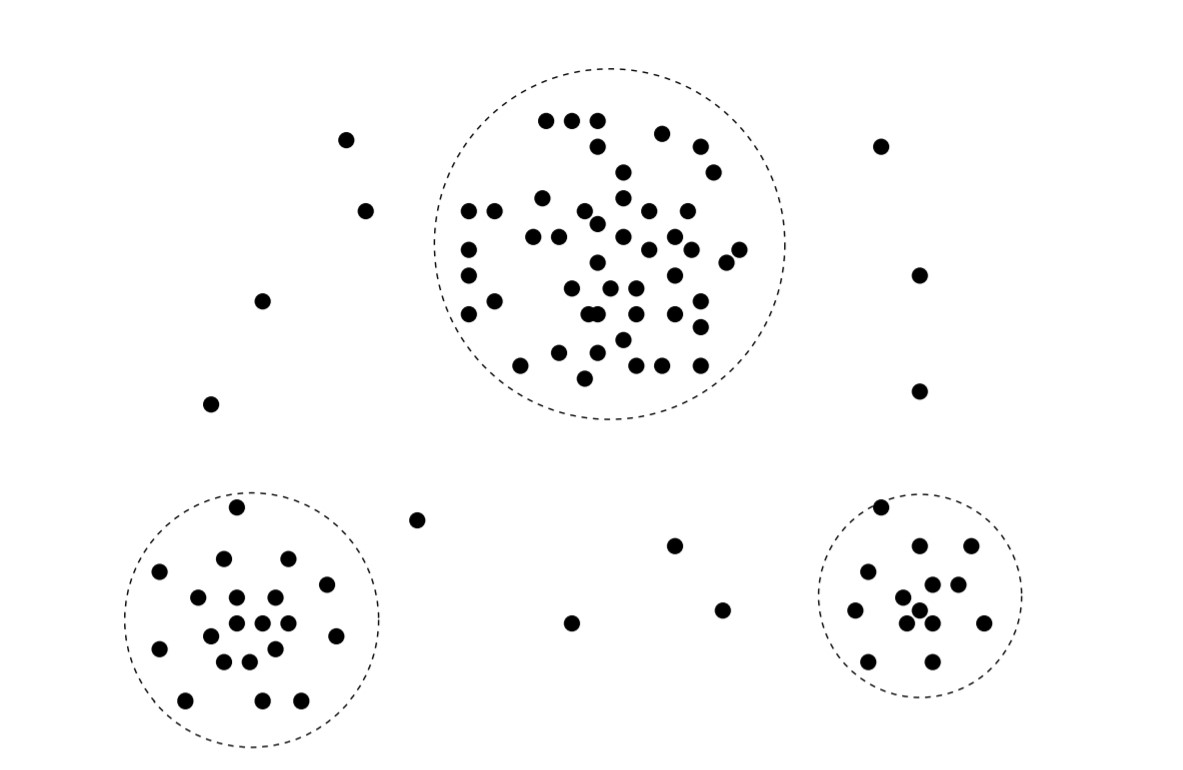
\includegraphics[scale=0.3]{clustering1}
	\caption{Hasil dari clustering}
	\label{fig:rnaalgorithm}
\end{figure}

\section{K-Means Clustering} 
K-Means Clustering akan mempartisi data pada dataset D ke dalam k buah cluster 
$(C_1, \ldots, C_k)$, dengan syarat $C_i \subset D$ dan $C_i \cap C_j = \emptyset$ untuk $(1 \leq i, j \leq k)$.  K-Means Clustering memiliki fungsi obyektif untuk menilai kualitas partisi sehingga tuple-tuple di dalam sebuah cluster akan mirip satu sama lain dan berbeda dengan tuple-tuple di kluster lain. K-Means Clustering bertujuan untuk mencari tingkat kesamaan dalam satu cluster yang tinggi, dengan tingkat kesamaan dengan kluster lain yang rendah.

\par K-Means Clustering menggunakan centroid dari cluster $(C_i)$  untuk mewakili kluster tersebut. Centroid adalah pusat massa sebuah cluster sebagai titik pusatnya. Centroid dapat didefinisikan dengan berbagai cara seperti dengan rata-rata nilai atribut pada sebuah cluster. Perbedaan antar objek diukur berdasarkan jarak antar objek p dengan centroidnya, diwakili dengan notasi Dist$(p, C_i)$. Notasi Dist$(p,C_i)$ adalah Euclidean distance antara dua titik p dan $C_i$. Untuk setiap tuple di setiap cluster, jarak dari tuple ke pusat clusternya akan dikuadratkan dan dijumlah. Kualitas sebuah cluster dapat diukur berdasarkan jumlah variasi di dalam kluster itu sendiri. Semakin banyak variasi dalam sebuah kluster, maka akan semakin buruk kualitas kluster tersebut.

\par Mengoptimalkan jumlah variasi pada kluster merupakan tantangan komputasi. Dalam kasus terburuk, perlu mencoba sejumlah kemungkinan partisi (p) yang eksponensial terhadap jumlah cluster (C) dengan kompleksitas $(p^C)$ dan memeriksa nilai variasi di dalam sebuah kelompok data. Telah terbukti bahwa K-Means Clustering termasuk masalah eksponensial walaupun memiliki jumlah kluster yang sedikit. Jika jumlah kluster dan dimensi ruang pada kluster diperbaiki, masalah dapat diselesaikan dalam waktu O (n dk + 1 log n), di mana n adalah jumlah tuple,dk adalah jumlah dimensi ruang pada kluster. Untuk mengatasi biaya komputasi yang mahal, solusi yang tepat adalah menggunakan pendekatan algoritma greedy. Salah satu contoh penerapan algoritma greedy adalah, Greedy K-Member Clustering.\\
\\
\noindent Secara singkat, langkah kerja algoritma K-Means Clustering dapat dijelaskan sebagai berikut:
\begin{enumerate}
\item Memilih jumlah cluster (K).
\item Inisialisasi K-buah nilai centroid secara random.
\item Menghitung kemiripan antar objek dengan menghitung jarak terdekat antar suatu objek dengan centroid. Jika suatu objek memiliki jarak terpendek dengan nilai centroid tertentu maka objek tersebut akan dikelompokkan pada kelompok centroid tersebut.
\item Menentukan nilai centroid baru dengan cara menghitung nilai rata-rata dari semua objek pada kelompok tertentu.
\item Kumpulan objek pada setiap cluster dikelompokkan kembali berdasarkan nilai centroid baru.
\item Ulangi langkah 3 dan 4 sampai nilai centroid tidak mengalami perubahan atau Thresshold.
\end{enumerate}

\begin{figure}[H]
	\centering
	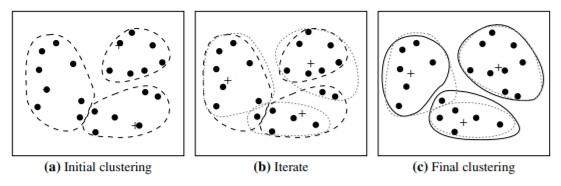
\includegraphics[scale=0.8]{kmeansclustering1}
	\caption{K-Means Clustering}
	\label{fig:rnaalgorithm}
\end{figure}


\section{Bidang Terkait Data Mining}
Data mining terhubung dengan beberapa bidang lain seperti statistika, machine learning, pengenalan pola, sistem basisdata, sistem data warehouse, information retrieval, visualisasi data, dan bidang lainnya. Jenis bidang ini memberikan berkontribusi yang signifikan terhadap keberhasilan dalam pengolahan data menggunakan teknik data mining.

\begin{figure}[H]
	\centering
	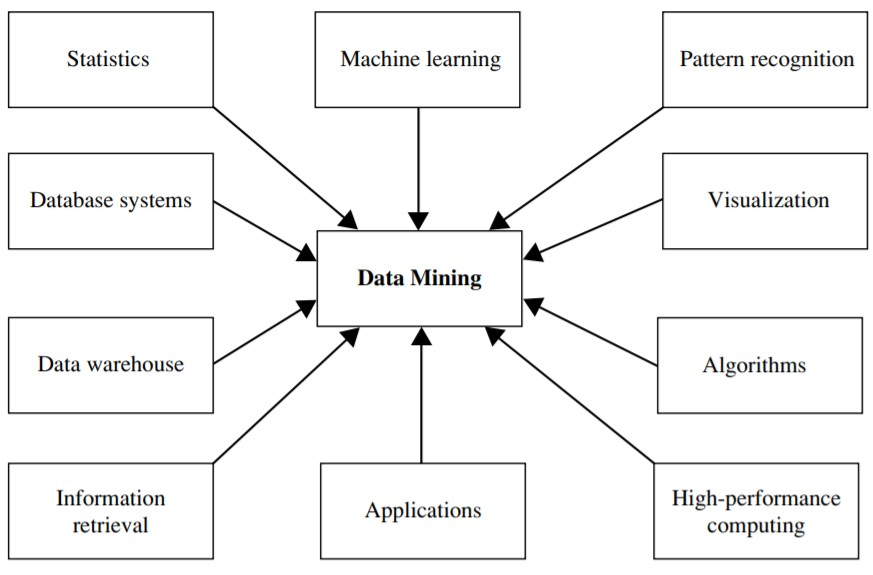
\includegraphics[scale=0.5]{teknologidatamining1}
	\caption{Jenis bidang terkait data mining}
	\label{fig:rnaalgorithm}
\end{figure}

\subsection{Visualisasi Data} 
Visualisasi adalah penggunaan representasi data pada komputer. Visualisasi data melibatkan penyajian data dalam bentuk grafik atau gambar agar membuat informasi mudah dimengerti, membantu menjelaskan fakta, dan menentukan arah tindakan. Sulit untuk membuat visualisasi pada ukuran data yang besar. Kemampuan untuk memvisualisasikan data sangat penting untuk melakukan analisis data. Saat ini, komputer dapat memproses data dalam jumlah besar. Visualisasi data berkaitan dengan tata cara untuk menyatakan representasi data secara informatif agar mudah untuk dipahami. Dengan adanya representasi data dalam bentuk visual, seseorang dapat memahami sekumpulan data dengan mudah. Hal ini membantu individu  menemukan pola, memahami informasi, dan membentuk opini berdasarkan hasil analisis. Visualisasi menguntungkan bidang studi yang membutuhkan cara-cara inovatif untuk menyajikan informasi yang besar dan kompleks. Dalam visualisasi data, data diabstraksi dan diringkas. Visualisasi harus melakukan reduksi data, melakukan ransformasi data, dan menampilkan hasil pengolahan data dalam bentuk grafik. Grafik dapat menyajikan hasil analisis data agar mudah untuk dimengerti.
\\\\
Beberapa teknik visualisasi yang umum digunakan untuk menggambarkan informasi dari sekumpulan data adalah berikut:

\begin{itemize}
\item Line chart adalah grafik pembanding perubahan nilai atribut pada periode waktu tertentu.
\item Bar chart adalah grafik pembanding nilai atribut untuk jenis kategori yang berbeda.
\item Scatter plot adalah grafik dengan plot dua dimensi yang menunjukkan variasi dua item.
\item Pie chart adalah grafik untuk membandingkan persentase nilai atribut secara keseluruhan.
\end{itemize}

\subsection{Statistika}
Statistika adalah suatu metode yang digunakan dalam pengumpulan dan analisis data dapat diperoleh informasi yang bermamfaat. Statistika menyedikan prinsip dan metodologi untuk merancang proses pengumpulan data , meringkas dan menyajikan data yang telah diperoleh , menganalisis dan pengambilan keputusan secara ringkas. Secara ringkas pengertian statistika adalah pengetahuan yang berkaitan dengan pengumpulan angka-angka , pengolahan , dan penganalisisan , penarikan kesimpulan , serta pembuatan keputusan berdasarkan data dan fakta yang sudah dianalisis.

Analisis statistika secara deskriptif merupakan metode penyajian data sehingga memberikan informasi yang berguna. Upaya penyajian ini dimaksudkan untuk mengungkapkan informasi penting yang terdapat dalam data ke dalam berntuk yang lebih ringkas dan sederhana yang pada akhirnya mengarah pada keperluan adanya penjelasan dan penafsiran (Aunudin, 1989). Analisis yang dilakukan dalam statistika meliputi ukuran pemusatan dan penyebaran data. Ukuran pemusatan data meliputi nilai rata-rata (mean), modus, dan median. Sedangkan ukuran penyebaran data meliputi variansi dan standar deviasi

\subsubsection{Mean}
Mean adalah nilai rata-rata dari sekumpulan data. Nilai dari mean dapat ditentukan dengan cara membagi jumlah data yang ada dengan total data. Mean terdiri dari dua jenis yaitu: populasi dan sampel. Mean populasi memiliki simbol $\mu$, sedangkan mean untuk sampel memiliki simbol $\overline{x}$.   
\\\\
Berikut adalah rumus untuk menghitung mean populasi ($\mu$):

\begin{equation}
\mu = \frac{x_1+x_2+x_3+\ldots+x_n}{N}
\end{equation}

\noindent Berikut adalah rumus untuk menghitung mean sampel ($\overline{x}$):

\begin{equation}
\overline{x} = \frac{x_1+x_2+x_3+\ldots+x_n}{N}
\end{equation}


\subsubsection{Median}
Median menentukan letak dari titik tengah data setelah data disusun menurut urutan nilainya. Median disimbolkan dengan $\widetilde x$. Median dibedakan  berdasarkan jumlah datanya, yaitu jumlah data yang bernilai ganjil dan jumlah data yang bernilai genap. 
\\\\
\noindent Berikut adalah rumus untuk menghitung median dengan jumlah data yang bernilai ganjil dan genap:

\begin{align}
\widetilde x = 
\left\{ \begin{array}{cc} 
X_{\frac{n+1}{2}} & \hspace{5mm} ,n=ganjil \vspace{2mm}\\
\frac{X_{\frac{n}{2}}+X_{\frac{n}{2}+1}}{2}  & \hspace{5mm} ,n=genap \\
 \end{array} 
 \right.
\end{align}

\subsubsection{Modus}
Modus adalah nilai yang sering muncul dalam kelompok data tersebut. Modus berarti nilai data yang memiliki frekuensi terbanyak dalam sekelompok data. Jika dalam suatu kelompok data memiliki lebih dari satu nilai data yang sering muncul maka sekumpulan data tersebut memiliki lebih dari satu modus. Sekelompok data yang memiliki dua modus disebut dengan bimodal, sedangkan jika lebih dari dua modus disebut multimodal. Jika dalam sekelompok data tidak terdapat satu pun nilai data yang sering muncul, maka sekelompok data tersebut dianggap tidak memiliki modus. Modus biasanya dilambangkan dengan $M_o$.



\subsection{Machine Learning} 
Machine learning mempelajari metode pembelajaran pada sebuah komputer, agar dapat belajar secara mandiri atau meningkatkan kinerjanya berdasarkan data pelatihan yang pernah diberi. Penelitian terutama pada machine learning adalah membuat program komputer secara otomatis belajar mengenali pola yang kompleks dan membuat keputusan cerdas berdasarkan data. Machine leaning adalah disiplin ilmu yang berkembang dengan cepat. Berikut adalah jenis pembelajaran machine learning untuk mengenali sebuah pola:

\par Contoh penerapan metode machine Learning adalah supervised learning. Supervised learning  adalah permasalahan klasifikasi. Beberapa algoritma klasifikasi yang umum digunakan adalah regression, , artificial neural networks, and random forests. Tujuan klasifikasi adalah untuk mengenali hubungan yang spesifik dalam data input agar secara efektif dapat menghasilkan data output yang benar apabila diberikan data baru. Menentukan output yang benar pada klasifikasi ditentukan dari banyaknya data pelatihan yang diberi. Noisy data  sering ditemui pada banyak kasus sehingga perlu ditangani secara khusus dengan metode machine learning tertentu.

\par Contoh penerapan lain dari metode machine learning adalah unsupervised learning. Unsupervised learning adalah permasalahan pengelompokan/clustering. Unsupervised learning mempelajari sifat data tanpa menggunakan label yang disediakan secara eksplisit. Beberapa algoritma clustering yang umum digunakan adalah k-means clustering. Karena tidak ada label yang disediakan, perlu adanya cara khusus untuk mencari kesamaan antar nilai atribut data menggunakan metode unsupervised learning.

\section{Privacy Preserving Data Mining (PPDM)} 
Privacy Preserving Data Mining (PPDM) adalah teknik yang telah dikembangkan untuk mencegah pengungkapan informasi sensitif seseorang saat dilakukan data mining dari sekumpulan data yang berukuran besar. PPDM dapat melakukan perubahan dan  menghilangkan sebagian data untuk menjaga privasi. Semakin banyak terjadinya perubahan pada data, maka perlindungan privasi akan meningkat dan kualitas informasi akan menurun.  Utilitas adalah kondisi untuk meningkatkan kualitas informasi yang diperoleh dengan mempertimbangkan jumlah data yang dimodifikasi. Metode PPDM menjamin perlindungan data pada tingkat privasi tertentu bersamaan dengan memaksimalkan utilitas data, sehingga memungkinkan pengolahan data mining menghasilkan informasi yang efektif. Klasifikasi PPDM dibuat berdasarkan siklus pengolahan data mulai dari pengumpulan data, proses data mining, penerbitan data, dan distribusi data.

\subsection{Pengumpulan Data} 
Untuk memastikan privasi tetap terjada pada saat pengumpulan data, perangkat sensor sebagai reseptor input dapat mengacak nilai data yang ditangkap sebelum data dikirimkan kepada kolektor (perangkat lain). Entitas yang mengumpulkan data diasumsikan menjadi entitas yang tidak dapat dipercaya. Oleh karena itu, nilai-nilai data sesungguhnya tidak pernah disimpan dalam basis data, dan nilai-nilai tersebut hanya dapat digunakan setelah melalui tahap transformasi (saat proses KDD). Metode yang dapat digunakan untuk melindungi atribut sensitif saat pengumpulan data adalah randomisation.

\subsection{Proses Data Mining} 
Penambangan data sangat memungkinkan terjadinya identifikasi terhadap atribut sensitif. Berikut adalah beberapa metode yang dapat digunakan untuk melindungi atribut sensitif seseorang saat proses data mining yaitu: association rule hiding adalah aturan untuk mengekstraksi seluruh atribut non-sensitif, downgrading classifier effectiveness adalah teknik untuk menurunkan keakuratan dari classifier yang sering digunakan, query auditing and inference control adalah aturan yang membatasi lingkup penggunaan kueri agregasi berdasarkan dataset, bukan terhadap catatan individu atau kelompok tertentu.

\subsection{Publikasi Data} 
Ada kondisi di mana sebuah perusahaan ingin melakukan publikasi koleksi data baik secara publik atau kepada pihak ketiga untuk analisis data tanpa mengungkapkan kepemilikan data sensitif. Dalam situasi ini, PPDM dapat dicapai dengan melakukan anonimisasi pada atribut data yang bersifat sensitif sebelum data tersebut dipublikasikan. PPDM pada publikasi data dikenal sebagai Privacy Preserving Data Publishing (PPDP). Berikut adalah beberapa metode yang dapat digunakan untuk melindungi atribut sensitif saat publikasi data yaitu: k-anonymity, l-diversity, t-closeness, e-differential privacy.

\subsection{Distribusi Data} 
Ada kondisi di mana seseorang berusaha untuk melakukan teknik data mining melalui data yang bersifat publik, berdasarkan ketehubungan nilai atribut non-sensitif. Beberapa pendekatan dapat digunakan untuk melindungi atribut sensitif saat distribusi data. Pendekatan pertama adalah menggunakan protokol yang aman untuk mencegah pengungkapan atau perhitungan informasi antar entitas seperti: oblivious transfer protocol dan homomorphic encryption.  Pendekatan kedua adalah mempertimbangkan sekumpulan operasi primitif yang sering digunakan pada algoritma data mining seperti: secure sum, secure set union, secure size of intersection, scalar product and the set intersection.

\section{Jenis Serangan Publikasi Data} 
Menurut Dalenius (1977), perlindungan privasi tidak akan memberikan kesempatan bagi orang lain untuk mendapatkan informasi sensitif spesifik dari seseorang atau individu meskipun orang lain mengetahui informasi umum yang berhubungan dengan informasi sensitif individu tersebut. Secara umum, orang lain dapat menemukan sebuah cara untuk memetakan sebuah data ke dalam tabel yang telah dianonimisasi ketika data tersebut telah dipublikasikan. Serangan ini dikenal dengan nama linkage attack. Model serangan ini dapat dikategorikan menjadi dua macam, berdasarkan jenis serangannya.

\subsection{Record Linkage}
Record linkage mengacu pada pemetaan beberapa data korban yang ditargetkan ke dalam sebuah tabel yang dirilis secara publik berdasarkan prinsip anonimisasi. Jika pada proses identifikasi salah satu nilai tupel cocok dengan nilai tupel lainnya pada tabel yang sudah dipublikasi, maka memungkinkan atribut sensitif miliki seseorang dapat diketahui oleh orang lain. Menggunakan pemodelan k-anonimity, terbukti dapat menghindari jenis serangan record linkage.

\subsection{Attribute Linkage} 
Dalam serangan ini, penyerang mendapatkan beberapa informasi terkait atribut sensitifnya, meskipun penyerang tidak dapat menghubungkan satu tupel dengan tupel lain dari data yang telah dipublikasi. Pemodelan  l-diversity dapat mencegah serangan attribute linkage. Kondisi yang diperlukan adalah kesetaraan setidaknya sebuah tupel memiliki l nilai atribut yang berbeda dengan tupel lainnya pada data yang telah dipublikasi. Konsep dasarnya adalah menghindari hubungan atribut jika akan ada nilai sensitif yang bernilai unik pada tupel-tuper tertentu dalam sebuah tabel.

\section{Anonimisasi}
Anonimisasi adalah proses menghilangkan pengidentifikasi pribadi, baik langsung maupun tidak langsung, yang dapat menyebabkan seseorang diidentifikasi. Seseorang dapat diidentifikasi secara langsung dari nama, alamat, kode pos, nomor telepon, foto atau gambar, atau beberapa karakteristik pribadi unik lainnya. Seseorang dapat diidentifikasi secara tidak langsung ketika informasi tertentu dihubungkan bersama dengan sumber informasi lain.
\\\\
Berikut adalah istilah yang umum digunakan pada proses anonimisasi data: 

\begin{itemize}
\item Identifier (ID) adalah atribut yang unik dan secara langsung dapat mengidentifikasi seseorang seperti nama, nomor ID, dan nomor ponsel.
\item Quasi-Identifier (QID) adalah kombinasi atribut yang mungkin terjadi untuk mengidentifikasi individu berdasarkan penggabungan informasi lain dari luar. Seluruh atribut data terkecuali atribut identifier dapat dianggap sebagai atribut quasi-identifier.
\item Equivalence class (EQ) adalah himpunan tupel 
dengan jenis nilai atribut yang identik satu sama lain.
\item Sensitive Attribute (SA) adalah atribut yang menyangkut informasi privasi sensitif seseorang.
\item Non-sensitive Attribute (NSA) adalah atribut yang tidak menyangkut informasi privasi sensitif seseorang.
\end{itemize}


\subsection{Anonimisasi berdasarkan generalisasi dan supresi}
Idenya adalah meningkatkan jumlah equivalence class pada tabel dengan mengurangi nilai akurasi data dari atribut quasi-identifier. Secara umum, quasi-identifier dapat dibagi menjadi dua jenis yaitu atribut numerik dan atribut kategori. Atribut numerik biasanya dilakukan generalisasi secara interval, misalnya, usia 16 dapat digeneralisasi ke interval [10-20]. Dan untuk atribut kategori, nilai-nilai  asli akan digantikan oleh yang nilai lebih umum menurut VGH. Sebagai contoh, atribut negara yang nilainya "China", maka dapat digeneralisasi menjadi "Asia". Supresi dapat dipandang sebagai bentuk generalisasi yang ekstrem, di mana atribut yang digeneralisasi tidak dapat digeneralisasi lebih lanjut.

\subsection{Anonimisasi berdasarkan generalisasi}
Saat ini, banyak jenis algoritma yang dipakai untuj implementasi algoritma anonimisasi, dan sebagian besar algoritma menggunakan pendekatan generalisasi dan supresi untuk proses anonimisasi. Berdasarkan perspektif, metode generalisasi dapat dibagi menjadi 2 kategori yaitu global generalization dan local generalization. 

\subsubsection{Global generalization}
Algoritma ini memungkinkan seluruh domain atribut identifier dipetakan ke dalam domain generalisasi, artinya nilai dalam tabel hanya akan memiliki satu nilai. Secara umum, algoritma global generalization dapat diimplementasi secara sederhana dan efisien. Akan tetapi perlu diketahui bahwa generalisasi yang berlebihan dapat menyebabkan hilangnya informasi yang tinggi. 

\subsubsection{Local generalization}
Algoritma ini memetakan seluruh nilai atribut ke dalam nilai generalisasi berdasarkan pengelompokan. Pengelompokan nilai atribut yang sama dapat digeneralisasikan ke nilai atribut yang berbeda jika berada dalam kelompok yang berbeda. Pengelompokan data biasanya mengadopsi beberapa prinsip heuristik, seperti pembagian, pengelompokan, dan sebagainya. Jumlah kehilangan informasi pada jenis algoritma ini lebih kecil dibandingkan dengan algoritma global generalization. Akan tetapi algoritma ini memiliki kompleksitas yang lebih tinggi dibandingkan dengan algoritma global generalization. Dalam kasus sejumlah besar data, kompleksitas adalah masalah yang harus diperhatikan. 
\\\\
Melalui pernyataan diatas, dapat disimpulkan bahwa secara umum algoritma generalisasi global paling efisien, tetapi kualitas informasinya rendah. Sebaliknya, algoritma generalisasi lokal dapat sangat meningkatkan kualitas informasi, tetapi memiliki kompleksitas yang tinggi sehingga tidak efisien. 

\subsection{Anonimisasi berdasarkan clustering}
Anonimisasi dapat diimplementasikan dengan pengelompokan/clustering. Clustering merupakan metode yang paling umum digunakan. Ide dasarnya adalah untuk menghasilkan setidaknya k buah tupel kelas sebagai kelas ekivalensi. Tupel dalam kelas yang sama harus sama mungkin untuk membuat kehilangan informasi seminimal mungkin setelah generalisasi. Konsep anonimisasi berdasarkan clustering ada ide dasar untuk perancangan model K-anonimity.

\newpage
\section{K-Anonymity}
K-anonymity merupakan model yang paling efektif untuk melindungi privasi saat melakukan publikasi data. K-anonymity adalah pemodelan untuk mengurangi perbedaan antara satu data dengan data lain, agar sebuah data tidak dapat dibedakan setidaknya dengan k-1 data lainnya. Dengan kata lain, penyerang tidak dapat mengidentifikasi identitas dari satu data karena k-1 data yang lain memiliki sifat yang sama. Dalam pemodelan k-anonymity, nilai k dapat digunakan sebagai tingkat keamanan privasi. Semakin tinggi nilai k, semakin sulit untuk mengindentifikasi sebuah data. Secara teori, probabilitas identifikasi sebuah data adalah 1 / k. Namun, meningkatkan nilai k juga berpengaruh terhadap nilai informasi yang diperoleh dari sekumpulan data.

\par K- anonymity pertama kali diusulkan pada tahun 1998 oleh Sweeney et al. K- anonymity tergantung pada menganonimkan kumpulan data asli untuk memenuhi persyaratan anonimisasi, yang dapat digunakan untuk penerbitan data. Teknik anonimisasi yang umum adalah generalisasi dan disembunyikan. Gagasan dasar K- anonymity adalah menganonimkan data penerbitan untuk memenuhi persyaratan bahwa setidaknya K tupel tidak dapat dibedakan satu sama lain. Yaitu, untuk masing-masing tuple terdapat setidaknya K tuple dengan nilai yang sama dari quasi-identifiers. Para peneliti telah membuktikan bahwa kompleksitas K- anonymity adalah NP-hard. NP-hard adalah istilah yang sering digunakan untuk menyatakan kompleksitas sebuah algoritma sangat tinggi (eksponensial).

\par Penelitian menunjukkan bahwa sebagian besar metode k-anonymity menggunakan metode generalisasi dan supresi. Pendekatan tersebut menderita kehilangan informasi yang signifikan karena mereka sangat bergantung terhadap hubungan relasi antar atribut. Oleh karena itu, hasil anonimisasi menghasilkan nilai kehilangan informasi yang cukup tinggi. Selain itu, algoritma anonimisasi yang ada hanya berfokus pada perlindungan informasi pribadi dan mengabaikan utilitas data yang sebenarnya. Akibatnya, nilai utilitas pada data yang telah dianonimisasi memiliki bernilai rendah. Beberapa algoritma telah dicoba untuk mengimplementasikan pemodelan k-anonymity.

\par Algoritma k-means clustering akan melakukan beberapa iterasi sampai centroid dari semua data tidak lagi berubah atau perubahannya kecil. Algoritma k-means clustering tidak mampu untuk menyelesaikan masalah pada atribut yang bernilai kategorikal. Kelebihan dari algoritma k-means clustering adalah memiliki hasil pengelompokan yang sudah baik. Kekurangan dari algoritma k-means clustering adalah pemilihan centroid awal k-means secara acak, sehingga setelah digeneralisasi hasil pengelompokannya mengakibatkan hilangnya informasi yang besar.

\par Algoritma k-member dapat melakukan generalisasi atribut kategorikal dengan memperoleh kualitas informasi yang lebih baik daripada algoritma k-means clustering. Namun algoritma k-member masih memiliki masalah ketika melakukan pengelompokan data. Kekurangan dari algoritma K-member adalah hanya mempertimbangkan pengelompokan terakhir tanpa memperhatikan pengelompokan yang dihasilkan pada proses sebelumnya sehingga menyebabkan distribusi kelompok pada beberapa bagian menjadi kurang tepat. 

\par Untuk menghindari kekurangan pada algoritma k-means dan algoritma k-member maka kedua konsep ini perlu digabung menjadi sebuah algoritma baru dengan nama algoritma Greedy K-member Clustering. Algoritma Greedy K-member Clustering mendapatkan hasil pengelompokan yang lebih tepat dan memiliki nilai informasi yang lebih baik meskipun dilakukan generalisasi. Menggunakan algoritma Greedy K-Member Clustering, pengelompokan data dapat dilakukan satu kali sehingga dapat menurunkan kompleksitas algoritma dan hasil  pemilihan centroid dapat dioptimalkan sehingga hasil pengelompokan dapat ditingkatkan secara signifikan. 

\newpage
\section{Greedy K-Member Clustering}
Penelitian menunjukkan bahwa sebagian besar metode k-anonymity didasarkan pada generalisasi dan teknik penekanan sehingga menderita dari kehilangan informasi yang signifikan. Masalah pengelompokan dapat meminimalkan kehilangan informasi. Akan tetapi k-member clustering berpotensi memiliki kompleksitas eksponensial. Untuk menurunkan kompleksitas, maka permasalahan pengelompokan pada algoritma k-member dapat didefinisikan sebagai permasalahan greedy. Algoritma Greedy K-Clustering anggota bertujuan untuk membagi seluruh tuple pada dataset ke masing-masing cluster dengan kerumitan yang lebih baik dan mendukung informasi yang lebih banyak dibandingkan algoritma clustering yang lain.

\begin{theorem}
Masalah pengambilan keputusan pada k-member clustering adalah NP-complete.
\end{theorem}

\begin{proof}
Melalui pengamatan Aggarwal et al, permasalahan k-member clustering dapat diselesaikan dengan kompleksitas polinomial.
\end{proof}

\begin{theorem}
N adalah total tuple dan k adalah parameter anonimisasi. Setiap kluster yang ditemukan oleh algoritma greedy k-member clustering memiliki jumlah tuple minimal sebanyak k, dan jumlah tuple tidak melebihi $2k–1$.
\end{theorem}

\begin{proof}
S adalah himpunan tuple. Algoritma ini menemukan cluster selama jumlah tuple yang tersisa sama dengan atau lebih besar dari k, setiap cluster berisi k tuple. Jika total tuple pada S kurang dari k, maka sisa tuple akan dikelompokan pada kelompok kluster yang sudah ada. Oleh karena itu, ukuran maksimum sebuah cluster adalah $2k - 1$.
\end{proof}

\begin{theorem}
N adalah jumlah tuple dan k menjadi parameter anonimitas yang ditentukan. Jika $n \gg k$, kompleksitas algoritma greedy k-member clustering adalah $O(n^2)$.
\end{theorem}

\begin{proof}
Algoritma greedy k-member clustering menghabiskan sebagian besar waktunya untuk memilih tuple dari S satu per satu hingga mencapai $|S| = k$. Karena ukuran set input berkurang satu pada setiap iterasi, total waktu eksekusi adalah O $(n^2)$.
\end{proof}

\noindent Secara singkat, langkah kerja algoritma Greedy K-Means Clustering dapat dijelaskan sebagai berikut:

\begin{enumerate}
\item Menghitung jumlah kluster (m) berdasarkan m = pagardalam(n/k)-1
\item Memilih sebuah tupel r secara acak, menjadikan r sebagai centroid dari kluster ci. 
\item Setiap (1-r) tupel dalam dataset S, akan dihitung distance antara (1-r) tupel lain dengan centroid r, lalu dipilih sebuah tupel dengan nilai distance terbesar pada centroid r, sehingga centroid r menjadi nilai centroid baru bagi kluster ci.
\item Memilih k-1 tupel lain yang dekat dengan nilai ri, artinya mencari nilai $IL(e1 \cup {rj})$ yang minimal.
\item Mengulangi langkaH 4, sampai pada kondisi dimana $|ci| < k$.
\item Mengulangi proses clustering dari tahap 3 sampai dengan tahap 5, sampai pada kondisi dimana $|S| < k$.  
\item Melakukan iterasi $(1-r)$ tupel yang tersisa dalam dataset dan masukan setiap tupel ke dalam sebuah kluster dengan mempertimbangkan nilai information loss seminimal mungkin. 
\end{enumerate}

\noindent Berikut adalah pseudocode secara lengkap dari algoritma greedy k-member clustering:

\begin{algorithm}[H]
  \caption{Find Best Record}\label{euclid}
  \begin{algorithmic}[1]
  %-------------- Input & Output -----------------
  \State \textbf{Function} \texttt{find\_best\_record(S,c)}
  \State \textbf{Input:} a set of records S and a cluster c.
  \State \textbf{Output:} a record r $\in$ S such that $IL(c \cup \{r\})$ is minimal
  \\
  %-------------- Baris 1-3 -----------------
  \State{$n = |S|$}
  \State{$min = \infty$}
  \State{$best = null$}
  \For{$i = 1 \ldots n$}
  \State{r = i-th record in S}
  \State{diff = $IL(c \cup \{r\}) - IL(c)$}
  \If{diff < min}
  \State{min = diff}
  \State{best = r}
  \EndIf
  \EndFor
  \State{return best}
  \end{algorithmic}
\end{algorithm}

\begin{algorithm}[H]
  \caption{Find Best Cluster}\label{euclid}
  \begin{algorithmic}[1]
  %-------------- Input & Output -----------------
  \State \textbf{Function} \texttt{find\_best\_cluster(C,r)}
  \State \textbf{Input:} a set of cluster C and a record r.
  \State \textbf{Output:} a cluster c $\in$ C such that $IL(c \cup \{r\})$ is minimal
  \\
  %-------------- Baris 1-3 -----------------
  \State{$n = |C|$}
  \State{$min = \infty$}
  \State{$best = null$}
  \For{$i = 1 \ldots n$}
  \State{r = i-th record in S}
  \State{diff = $IL(c \cup \{r\}) - IL(c)$}
  \If{diff < min}
  \State{min = diff}
  \State{best = c}
  \EndIf
  \EndFor
  \State{return best}
  \end{algorithmic}
\end{algorithm}

\begin{algorithm}[H]
  \caption{Greedy K-Member Clustering}\label{euclid}

  \begin{algorithmic}[1]
  %-------------- Input & Output -----------------
  \State \textbf{Function} \texttt{greedy\_k\_member\_clustering(S,k)}
  \State \textbf{Input:} a set of records S and a threshold value k
  \State \textbf{Output:} a set of clusters each of which contains at least k records.
  \\
  %-------------- Baris 1-3 -----------------
  \If{$S \leq k$} 
  \State{return S}
  \EndIf
  \\
  \State{$result = \phi$}
  \State{r = a randomly picked record from S}
  \While{$|S| \geq k$}
  \State{r = the furthest record from r}
  \State{S = S - \{r\}}
  \State{c = \{r\}}
  	\While{$|c| < k$}
	\State{$find_best_record(S,c)$}  
	\State{S = S - \{r\}}
  	\State{c = c $\cup$ \{r\}}
  	\EndWhile
  	\State{result = result $\cup$ \{c\}}
  \EndWhile
  \While{$S \neq 0$}
  \State{r = a randomly picked record from S}
  \State{S = S - \{r\}}
  \State{$find_best_cluster(result,r)$}
  \State{c = c $\cup$ \{r\}}
  \EndWhile
  \State{return result}
  \end{algorithmic}
\end{algorithm}



\section{Hierarchy Based Generalization} 


Hierarchy-based generalization adalah tahapan anonimisasi setelah data yang memiliki quasi-identifier yang sama dikelompokan ke dalam kelas yang sama. Hierarchy-based generalization menggunakan konsep generalisasi dan supresi dalam melakukan anonimisasi. Hierarchy-based generalization termasuk metode full-domain generalization. Full-domain generalization diusulkan oleh Samarati dan Sweeney untuk memetakan seluruh domain untuk masing-masing atribut quasi-identifier pada tabel ke domain yang lebih umum. Skema ini menjamin bahwa semua nilai atribut tertentu dalam V adalah milik domain yang sama. 

\par Pendekatan dalam kelas ini mensyaratkan bahwa strategi generalisasi dari setiap atribut dalam quasi-identifier harus ditentukan sebelumnya oleh Domain Generalization Hierarchy (DGH), merupakan kumpulan domain yang sepenuhnya menunjukkan atribut yang sesuai harus digeneralisasi dalam beberapa langkah. Berdasarkan DGH, seseorang dapat memperoleh Value Generalization Hierarchy (VGH), merupakan partisi dari urutan himpunan nilai. Pada Gambar \ref{fig:hierarchybasedgeneralization1}, diberikan contoh perbedaan generalisasi menggunakan DGH dan VGH untuk atribut kode pos pada gambar (a) dan (b), jenis kelamin pada gambar (c) dan (d), dan usia pada gambar (e) dan (f).

\par Masalah k-anonimisasi adalah menemukan cara generalisasi yang tepat untuk seluruh quasi-identifier, dengan memaksimalkan kualitas data (meminimalkan nilai Information Loss) yang diperoleh saat dilakukan proses data mining. Meskipun solusi optimal k-anonimisasi adalah eksponensial, penelitian sebelumnya telah menghasilkan algoritma yang efisien agar konsep k-anonimisasi dapat diterima karenan memiliki kompleksitas yang cukup baik. Pendekatan Hierarchy-based generalization memiliki beberapa batasan yang signifikan. Pertama, Hierarchy-based generalization menderita kehilangan informasi yang relatif tinggi karena melakukan generalisasi pada nilai atribut yang berbeda. Keterbatasan lain pada hierarchy-based generalization adalah bahwa utilitas data yang dianonimisasi sangat bergantung pada pemilihan kata. Hierarchy-based generalization bergantung pada pengetahuan pengguna terhadap pengertian kata dari domain tertentu, sehingga sulit untuk mendapat nilai utilitas data dengan hasil yang diharapkan.
\\
\begin{figure}[H]
	\centering
	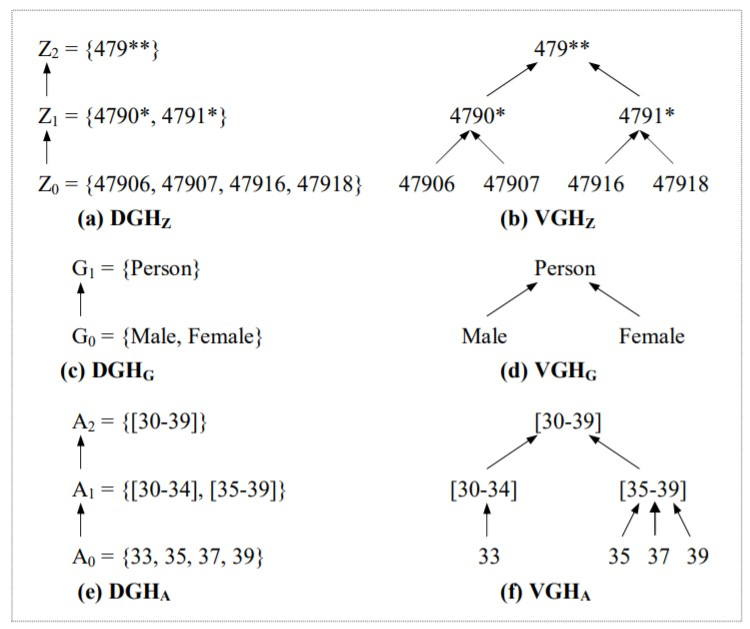
\includegraphics[scale=0.5]{hierarchybasedgeneralization1}
	\caption{Perbedaan DGH dan VGH}
	\label{fig:hierarchybasedgeneralization1}
\end{figure} 

\section{Distance, Information Loss, Cost Function} 
Konsep PPDM memberikan solusi untuk mengukur tingkat keamanan dan utilitas data berdasarkan data yang telah dianonimisasi menggunakan beberapa jenis metrik. Sebuah metrik tidak dapat mengukur performa algoritma, tingkat keamanan, dan utilitas data secara bersamaan. Untuk mengukur performa algoritma, tingkat keamanan, dan utilitas data secara bersamaan perlu menggunakan beberapa metrik. Beberapa metrik yang umum digunakan pada pengujian kualitas data yang telah dianonimisasi adalah distance,information loss, dan cost function.

\par Perlindungan privasi seringkali menurunkan utilitas informasi dari sebuah data. Metrik dipakai untuk mengukur banyaknya utilitas data yang hilang terhadap data yang telah dianonimisasi. Secara umum, pengukuran dilakukan dengan membandingkan hasil anonimisasi dengan dataset sesungguhnya. Beberapa atribut yang dapat diukur untuk menyatakan utilitas sebuah data adalah akurasi, kelengkapan, dan konsistensi. Akurasi dapat mengukur seberapa dekat data setelah dilakukan transformasi terhadap data asli. Kelengkapan dapat mencari data yang hilang dalam dataset setelah dilakukan transformasi. Konsistensi dapat menghitung jumlah korelasi yang hilang dalam dataset setelah dilakukan anonimisasi.

\subsection{Distance} 
Distance adalah salah satu perhitungan untuk menyatakan akurasi terhadap utilitas sebuah data. Distance merupakan faktor yang paling penting untuk menentukan hasil pengelompokan data. Pemilihan distance yang baik dapat mencapai hasil klasifikasi dengan lebih optimal. Atribut numerik dapat dihitung secara langsung menggunakan  Euclidean distance dan Manhattan distance. Distance tidak mampu menangani atribut kategorikal yang bertipe String. 

\par Perhitungan distance dipakai untuk mengukur tingkat perbedaan nilai antara dua jenis data yang berbeda. Perhitungan distance dilakukan berdasarkan pengelompokan tipe data numerik atau kategorikal. Karena masalah k-anonimitas menggunakan atribut numerik dan kategorikal, maka membutuhkan cara khusus untuk mengitung distance dari kedua jenis data pada saat yang sama. Distance ini dihitung berdasarkan representasi nilai numerik pada kelas ekivalensi yang sama. Dengan menggunakan metrik distance, seseorang dapat dengan mudah melakukan pembobotan dengan menambahkan bobot non-negatif untuk setiap atribut.

\subsubsection{Distance Data Numerik}
Untuk atribut numerik, perbedaan antara dua jenis data menggambarkan ketidaksamaan data. Ketika tupel dalam kelas ekivalensi yang sama digeneralisasi, quasi-identifier yang digeneralisasi harus merangkum semua nilai atribut dalam kelas ekivalensi. Generalisasi dua nilai x dan y dalam atribut numerik biasanya direpresentasikan sebagai rentang $[x,y]$ dimana $x < y$. Dengan demikian, perbedaan tersebut menangkap jumlah perbedaan yang disebabkan oleh proses generalisasi dari atribut masing-masing. Untuk menghitung distance pada atribut numerik, perlu mendefinisikan atribut |D|, dimana |D| adalah jumlah data pada sebuah domain berdasarkan satu atribut numerik. Distance atribut numerik yang sudah dinormalisasi berdasarkan nilai $vi, vj \in D$,  dapat dihitung menggunakan rumus dibawah ini:

\begin{equation}
\delta_n(v_1,v_2) = \frac{|v_1 - v_2|}{|D|} 
\end{equation}

\subsubsection{Distance Data Kategorial}
Untuk atribut kategorikal, distance tidak lagi berlaku karena sebagian besar domain kategorikal tidak dapat disebutkan dalam urutan tertentu. Solusi paling mudah adalah mengasumsikan setiap nilai dalam domain yang sama saling berbeda satu sama lain, misalkan jarak antara dua nilai adalah 0 jika kedua nilai bernilai sama, dan 1 jika kedua nilai bernilai beda. Beberapa domain mungkin memiliki beberapa hubungan semantik di antara nilai-nilai tersebut. Dalam domain seperti itu, diinginkan untuk mendefinisikan fungsi jarak berdasarkan hubungan yang ada. Hubungan seperti itu dapat dengan mudah ditangkap di pohon taksonomi. Kami berasumsi bahwa pohon taksonomi suatu domain adalah pohon seimbang yang simpul daunnya mewakili semua nilai berbeda dalam domain tersebut. Untuk beberapa jenis atribut, tidak ada hubungan semantik yang dapat membantu proses klasifikasi nilai domain. Asumsikan bahwa setiap nilai dalam domain yang sama, nilainya saling berbeda satu sama lain. Untuk mengakomodasi semua kasus ini, kami mendefinisikan fungsi jarak untuk nilai kategori sebagai berikut. Untuk menghitung distance pada atribut kategorikal, perlu mendefinisikan atribut |D| dan TD.|D| adalah jumlah data pada domain kategorikal. TD adalah taxonomy tree untuk domain D. Distance atribut kategorial yang sudah dinormalisasi berdasarkan nilai $vi, vj \in D$,  dapat dihitung menggunakan rumus dibawah ini:

\begin{equation}
\delta_C(v_1,v_2) = \frac{H(\Lambda(v_i,v_j))}{H(T_D)} 
\end{equation}


\subsection{Information Loss}
Information Loss (IL) digunakan untuk mengevaluasi seberapa baik kinerja algoritma k- anonimisasi terhadap utilitas sebuah data. Algoritma K-anonimisasi menyebabkan hilangnya sebagian besar informasi pada dataset. Information Loss (IL) menghitung ketersediaan data setelah melalui tahap anonimisasi secara akurat.  

\par Untuk menghitung Information Loss (IL), perlu mendefinisikan atribut: $e = {r_1,\ldots,r_k}$ adalah sebuah kluster dengan quasi-identifier yang terdiri dari atribut numerik {N1,. . . , Nm} dan atribut kategorikal ${C_1,\ldots,C_n}$. TCi adalah pohon taksonomi yang ditentukan untuk domain atribut kategorikal Ci. MINNi dan MAXNi adalah nilai minimum dan maksimum pada kluster e berdasarkan atribut Ni. $\cup C_i$ adalah sekumpulan nilai dalam kluster e berdasarkan atribut 
$C_i$. Perhitungan nilai Information Loss (IL) terhadap generalisasi kluster e, dilambangkan dengan IL (e). Information loss didefinisikan dengan rumus sebagai berikut:

\begin{eqnarray}
IL(e)&=& |e| \cdot D(e) \\
D(e) &=& \sum_{i=1}^{m} \frac{(MAX_{N_i} - MIN_{N_i})}{|N_i|} + \sum_{j=1}^{n}\frac{H(\Lambda(\cup_{C_j}))}{H(T_{C_j})}
\end{eqnarray}

\par Untuk menghitung total Information Loss,  E adalah set semua kelas ekivalensi kluster e pada tabel anonimisasi AT. Total Information Loss pada tabel AT dilambangkan dengan Total-IL(AT). Total Information Loss didefinisikan dengan rumus sebagai berikut:

\begin{equation}
Total-IL(AT) = \sum_{e \in \varepsilon}^{}  IL(e)
\end{equation}


\subsection{Cost Function} 
Cost function menyangkut efisiensi dan skalabilitas dari algoritma yang diterapkan. Metrik ini umum digunakan untuk menyatakan kualitas sebuah algoritma. Untuk mengukur efisiensi, seseorang dapat menggunakan standar untuk menentukan kompleksitas sebuah algoritma berdasarkan faktor waktu dan ruang. Waktu dapat diukur berdasarkan biaya komputasi algoritma. Ruang dapat diukur berdasarkan jumlah pemakaian memori selama menjalankan algoritma dari awal sampai dengan akhir. Kualitas sistem terdistribusi dapat diukur melalui biaya komunikasi antar komputer berdasarkan waktu,  jumlah pesan yang dipertukarkan, dan konsumsi bandwidth. 
 
\section{Sistem Terdistribusi}
Sistem terdistribusi adalah kumpulan komputer berjalan secara independen, yang saling terhubung dan saling bekerja sama untuk mencapai satu tujuan yang sama. Menurut Nora Jones (Netflix), sistem terdistribusi berbicara tentang sistem yang sangat rumit, yang terdiri dari banyak bagian yang saling berkomunikasi untuk menghasilkan produk tunggal. Menurut Brendan Burns (Microsoft), "Meningkatnya kekritisan pada sistem kini mengakibatkan munculnya ide pembangunan sistem distribusi untuk mengatasi masalah redundansi, memberikan toleransi kesalahan, dan menjamin tingkat ketersediaan yang tinggi". Beberapa konsep penting terkait sistem terdistribusi adalah setiap komputer bekerja untuk satu tujuan yang sama, setiap komputer mengerjakan tugas yang berbeda dengan komputer lainnya, pembagian jumlah tugas dilakukan secara adil, setiap komputer memiliki jalur komunikasi yang sama untuk saling bertukar informasi.
\\
\begin{figure}[H]
	\centering
	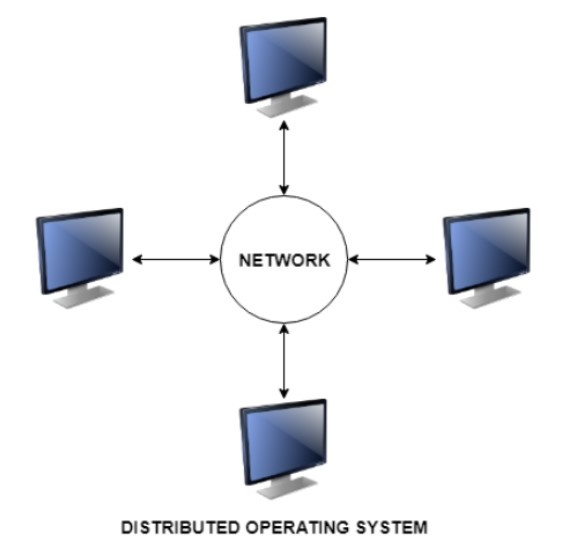
\includegraphics[scale=0.3]{sistemdistribusi1}
	\caption{Sistem Terdistribusi}
	\label{fig:rnaalgorithm}
\end{figure}

\subsection{Manfaat Sistem Terdistribusi}
Permasalahan sistem terdistribusi bukan difokuskan terhadap penggunaan sistem terdistribusi, melainkan alasan yang tepat untuk menggunakan sistem terdistribusi. Sistem terdistribusi dibutuhkan karena adanya peningkatan skala dalam pengolahan data dan munculnya sistem yang lebih handal untuk melakukan pemrosesan data. 
\\\\
Berikut adalah deskripsi dari manfaat penggunaan sistem terdistribusi bagi efektivitas pengolahan data:

\begin{itemize}
\item Horizontal Scalability\\
Sistem terdistribusi menawarkan kemampuan untuk  pemrosesan komputasi skala besar dengan murah

\item Reliability\\
Sistem terdistribusi dapat diandalkan karena proses komputasi pada sistem terdistribusi bergantung pada banyaknya komputer yang saling berkomunikasi satu sama lain untuk mencapai tujuan yang sama.
 
\item Performance\\
Sistem terdistribusi dapat menangani proses komputasi tugas secara efisien karena beban kerja sesungguhnya dibagi menjadi beberapa bagian dan tersebar di beberapa komputer. 
\end{itemize}

\subsection{Tantangan Sistem Terdistribusi} 
Manfaat penggunaan sistem terdistribusi adalah handal untuk pemrosesan data skala besar. Dalam perancangan sistem terdistribusi, sering ditemui kesulitan pada pemecahan masalah untuk kasus-kasus tertentu. 
\\\\
Berikut adalah tiga tantangan paling umum ditemui ketika merancang sistem terdistribusi:

\begin{itemize}
\item Penjadwalan\\
Kekuatan komputasi ada batasnya, sistem terdistribusi harus dapat memutuskan pekerjaan mana yang harus dijadwalkan untuk dijalankan dan menentukan prioritas pekerjaan yang dikerjakan lebih dulu. 
\item Latensi\\
Dengan pertukaran data yang semakin kompleks antara perangkat keras, perangkat lunak menggunakan jalur komunikasi jaringan, maka nilai latensi pada sistem tersebut menjadi sangat tinggi. Ketika volume data pada jaringan semakin meningkat, maka perlu dibuat partisi sementara untuk menyimpan data-data yang akan diolah. 
\item Observasi\\
Ketika sistem terdistribusi menjadi kompleks, kemampuan pengamatan untuk memahami kegagalan pada sistem terdistribusi merupakan tantangan besar. Pemantauan terhadap proses partisi data bermanfaat bagi sistem terdistribusi untuk menelusuri tingkat kegagalan proses pada setiap komputer. 
\end{itemize}

\newpage
\section{Big Data}
Big data adalah data yang besar dan kompleks sehingga tidak mungkin sistem tradisional dapat memproses dan bekerja pada lingkungan data yang besar secara maksimal. Big data dihasilkan oleh mesin dan manusia. Big data dapat dikategorikan menjadi data terstruktur, semi terstruktur dan tidak terstruktur. Big data tidak memungkinkan untuk dianalisis menggunakan kueri pada sistem manajemen basis data tradisional, karena waktu pemrosesan data terlalu lama.
\\\\
Sekumpulan data dapat dikatakan big data jika memenuhi  kelima sifat di bawah ini. Berikut adalah penjelasan kelima sifat yang dimiliki oleh big data:
\begin{itemize}
\item Volume\\
Volume menyajikan tantangan terbesar untuk melakukan analisis pada data yang besar. Banyak perusahaan memiliki sejumlah besar data yang diarsipkan, tetapi tidak memiliki kapasitas yang memadai untuk memproses data berukuran besar. Kemampuan memproses informasi pada data berukuran besar adalah daya tarik utama untuk menganalisis informasi untuk keperluan tertentu.
\item Velocity\\
Velocity mengacu pada peningkatan kecepatan ketika data dalam ukuran besar dihasilkan, sehingga membutuhkan peningkatan kecepatan pemrosesan, penyimpanan, dan analisis. Velocity selalu dikaitkan pada kecepatan dimana data baru selalui dihasilkan sepanjang waktu dan kecepatan perpindahan data.
\item Variety\\
Big data tidak selalu merupakan data terstruktur dan tidak mudah untuk mengolah data besar dengan format file yang beragan. Hal ini menunjukan bahwa keberagaman big data termasuk fakta yang sangat penting dan perlu diketahui untuk sebelum proses analisis data lebih lanjut. Berurusan dengan berbagai data terstruktur dan tidak terstruktur meningkatkan kompleksitas dalam menyimpan dan menganalisis big data. Sebagian besar data yang dihasilkan berbentuk data tidak terstruktur.
\item Veracity\\
Big data diperoleh dari berbagai macam sumber sehingga kebenaran sebuah data harus diuji. Kebenaran nilai sebuah data dapat teruji apabila mengambil sekumpulan data pada sumber yang terpecaya. Kualitas data yang ditangkap dapat sangat bervariasi. Sehingga keakuratan data yang dianalisis bergantung pada kebenaran nilai data berdasarkan sumber yang beragam.
\item Value\\
Value adalah aspek terpenting dalam big data. Potensial nilai yang terkandung dalam big data sangat besar. Sangat baik apabila dapat mengakses data-data pada big data, tetapi semuanya itu menjadi tidak berguna apabila data yang diperoleh tidak dapat diubah menjadi sebuah informasi terhadap masalah yang ingin diselesaikan. Value menjadi informasi yang sangat mahal karena memerlukan modal yang cukup besar untuk mengolah dan menyimpan data yang berukuran besar.
\end{itemize}

\newpage
\section{Analisis Big Data}
Analisis Big Data adalah proses menggunakan algoritma analisis yang berjalan pada platform pendukung yang kuat untuk mengungkap potensi yang disembunyikan dalam data besar, seperti pola tersembunyi atau korelasi yang tidak diketahui. Menurut
pemrosesan persyaratan waktu, analisis big data dapat dikategorikan ke dalam dua paradigma alternatif.
\\\\
Berikut adalah jenis analisis pada big data:
\begin{itemize}
\item 
Batch Processing\\
Paradigma batch processing adalah sekumpulan data disimpan terlebih dahulu, lalu pada waktu tertentu data yang telah terkumpul akan dilakukan analisis. MapReduce telah menjadi model penerapan batch processing pada umumnya. Ide dari MapReduce adalah  data yang besar dibagi menjadi potongan data yang lebih kecil. Selanjutnya, potongan-potongan data ini diproses secara paralel dan secara terdistribusi untuk dianalisis lebih lanjut. Hasil akhir dari MapReduce diperoleh dengan menggabungkan semua hasil dari setiap node. MapReduce menjadwalkan sumber daya komputasi secara dekat dengan lokasi data itu disimpan, sehingga dapat menghindari overhead dalam transmisi data. Konsep MapReduce banyak diterapkan dalam bioinformatika, data mining website, dan machine learning.

\item
Streaming Processing\\
Paradigma streaming processing adalah diasumsikan bahwa nilai informasi data yang diperoleh bergantung kepada seberapa cepat data dapat diolah secara real time. Pengertian dari real time adalah data diolah secara langsung ketika data tersebut diperoleh. Dalam paradigma ini, data diambil melalui aliran data. Karena aliran data yang masuk sangat cepat dan membawa volume yang cukup besar, maka hanya sebagian kecil data yang dapat disimpan dan diolah dalam memori yang terbatas. Teknologi streaming processing telah dipelajari selama beberapa dekade ini. Sistem pengolahan big data secara open source yaitu Spark dapat menerapkan paradigma ini. Paradigma streaming processing biasanya digunakan untuk analisis aplikasi online dalam tingkat satuan detik maupun milidetik.
\end{itemize}

\section{Hadoop}
Hadoop adalah framework yang melakukan pemrosesan data dengan memanfaatkan sistem terdistribusi dari kumpulan data besar yang terbagi pada seluruh  komputer. Hadoop dikembangkan oleh Google untuk penelitian pada sekumpulan data berukuran besar. Hadoop menggunakan bahasa pemrograman Java. Hadoop dirancang untuk memproses data dalam jumlah yang sangat besar dengan memanfaatkan penyimpanan pada hardisk. Karena pemrosesan pada Hadoop dilakukan berdasarkan paradigma batch processing, sehingga memerlukan waktu pemrosesan data tidak langsung. Hadoop melakukan replikasi file pada masing-masing node untuk menjamin reliability, availability, and fault tolerance.

\subsection{Ekosistem Hadoop}
\begin{figure}[H]
	\centering
	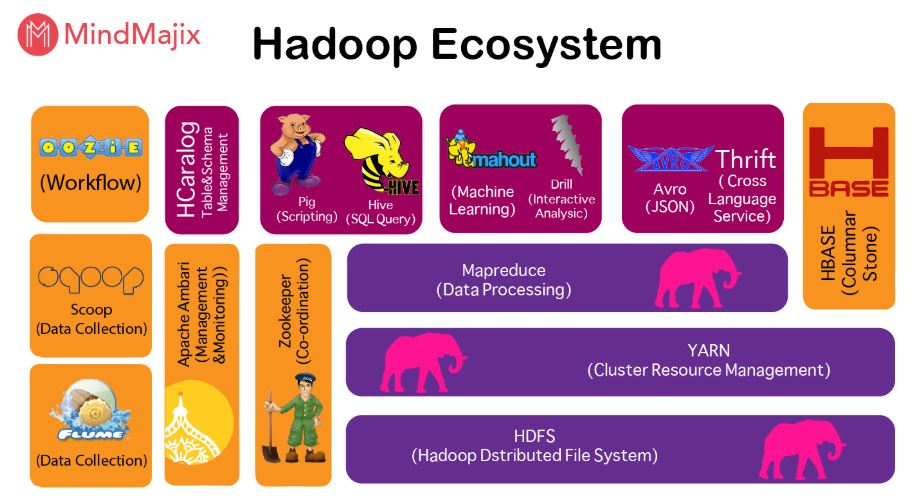
\includegraphics[scale=0.8]{hadoop_ecosystem}
	\caption{Ekosistem Hadoop}
	\label{fig:hadoop_ecosystem}
\end{figure}
Melalui Gambar \ref{fig:hadoop_ecosystem}, hadoop bekerja sama dengan teknologi lain untuk memenuhi berbagai macam kebutuhan dalam pengolahan big data. Masing-masing warna pada Gambar \ref{fig:hadoop_ecosystem} mewakili tingkat kebutuhan yang berbeda-beda. Warna ungu mewakili komponen pada Hadoop. Warna oranye mewakili teknologi tambahan yang umum digunakan secara bersamaan dengan hadoop. Warna ungu mewakili teknologi khusus yang digunakan secara bersamaan dengan hadoop untuk kasus-kasus tertentu.

\subsection{Arsitektur Hadoop}
\begin{figure}[H]
	\centering
	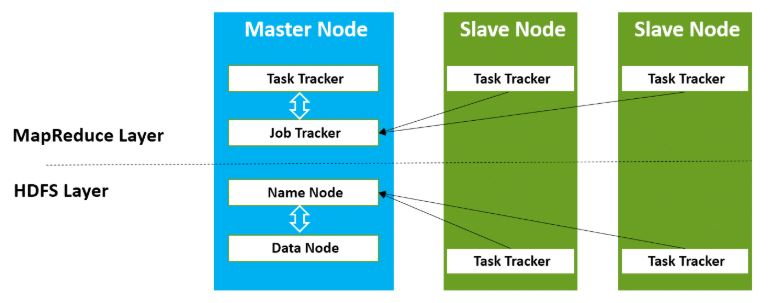
\includegraphics[scale=0.7]{arsitektur_hadoop}
	\caption{Arsitektur Hadoop}
	\label{fig:arsitektur_hadoop}
\end{figure}
Melalui Gambar \ref{fig:arsitektur_hadoop}, arsitektur Hadoop tersusun dari dua bagian utama yaitu MapReduce dan Hadoop Distributed File System (HDFS). Masing-masing bagian memiliki dua jenis node yaitu master node dan slave node. Master node mengatur jumlah pekerjaan yang diberikan kepada dirinya sendiri dan slave node. Slave node mengerjakan pekerjaan yang diberikan oleh master node.
\\\\
Hadoop terdiri dari empat elemen penting, yaitu:
\begin{enumerate}
\item NameNode
\item DataNode
\item JobTracker
\item TaskTracker
\end{enumerate}

\subsection{HDFS}
HDFS adalah sistem file terdistribusi pada Hadoop dengan menyediakan penyimpanan data yang handal, mendukung partisi, dan toleran terhadap kesalahan pada hardware. HDFS bekerja erat dengan MapReduce dengan mendistribusikan penyimpanan dan perhitungan di seluruh cluster dengan menggabungkan sumber daya penyimpanan yang dapat dipartisi tergantung kebutuhan. HDFS menerima data dalam format apa pun seperti teks, gambar, dan video. Keuntungan utama HDFS adalah memiliki toleransi terhadap kesalahan hardware. Dengan menyediakan transfer data cepat antara node dan memungkinkan Hadoop layanan yang cepat apabila terjadi kegagalan node, sehingga mengurangi risiko terhadao kegagalan komputasi. 
\\\\
Lapisan penyimpanan HDFS terdiri dari dua elemen:

\begin{itemize}
\item NameNode adalah sebuah komputer yang bertindak sebagai master node, sedangkan DataNode adalah komputer-komputer dalam Hadoop Cluster yang bertugas sebagai slaves atau anak buah. NameNode bertanggungjawab menyimpan informasi tentang penempatan block-block data dalam Hadoop Cluster. Ia bertanggungjawab mengorganisir dan mengontrol block-block data yang disimpan tersebar dalam komputer-komputer yang menyusun Hadoop Cluster. Sedangkan DataNode bertugas menyimpan block-block data yang dialamatkan kepadanya, dan secara berkala melaporkan kondisinya kepada NameNode.
\item DataNode bertugas menyimpan alamat block-block data, dan secara berkala melaporkan kondisinya kepada NameNode. DataNodes adalah elemen penyimpanan utama HDFS yang menyimpan blok data dan permintaan baca / tulis layanan pada file yang disimpan di HDFS. DataNode dikendalikan oleh NameNode. Blok yang disimpan dalam DataNodes direplikasi sesuai konfigurasi untuk memberikan keandalan dan ketersediaan tinggi. Blok yang direplikasi ini didistribusikan di seluruh cluster untuk memberikan perhitungan yang cepat.
\end{itemize}

\subsection{MapReduce}
MapReduce adalah kerangka kerja pemrograman untuk komputasi terdistribusi yang dibuat oleh Google menggunakan membagi dan menaklukkan metode untuk memecah masalah data besar yang kompleks menjadi unit-unit kecil pekerjaan dan memprosesnya
sejajar. Model pemrograman Map Reduce terdiri dari dua fungsi, yaitu Mapper dan Reducer. Pengguna dapat mengimplementasikan logika pemrosesan mereka sendiri dengan menentukan jenis atribut pada Mapper dan jenis pemrosesan untuk Reducer. Fungsi Mapper dibutuhkan
untuk menghasilkan daftar pasangan key,value. MapReduce akan mengelompokkan semua pasangan key,value dan meneruskannya kepada fungsi Reducer untuk mengolah data.

\newpage
\par Fungsi Mapper menerima input data berupa blok data dan menghasilkan output data berupa pasangan key-value. Hadoop membuat fungsi mapper untuk setiap blok data HDFS. Jumlah pemanggilan fungsi mapper sama dengan jumlah blok. Fungsi Reducer menerima input data berupa pasangan key-list value dan menghasilkan output data berupa pasangan key-value baru. Pemanggilan fungsi mapper dan fungsi reducer tidak saling bergantung satu sama lain karena komputasi dilakukan secara paralel. Jumlah pemanggilan fungsi reducer dapat ditentukan sesuai kebutuhan.

\begin{figure}[H]
	\centering
	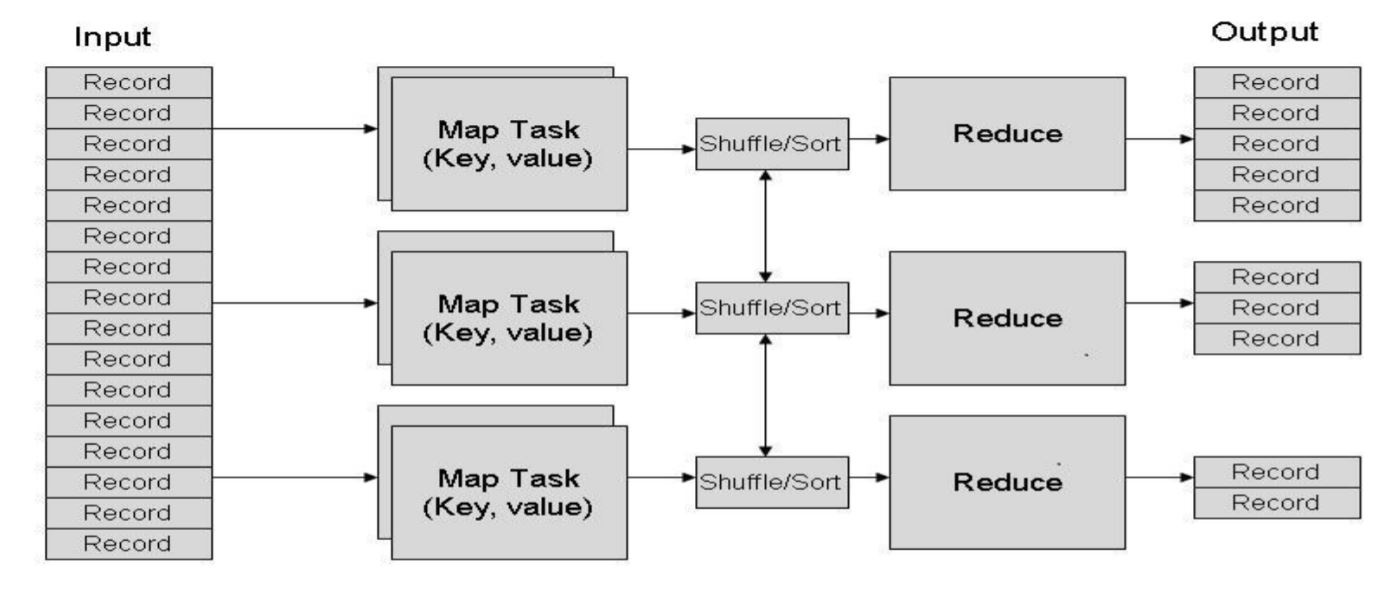
\includegraphics[scale=0.5]{MapReduceImage}
	\caption{Tahapan pada MapReduce}
	\label{fig:MapReduceImage}
\end{figure}


Pada Gambar \ref{fig:MapReduceImage}, tahapan MapReduce dapat dibagi menjadi dua fungsi utama:
\begin{itemize}
\item Mapper\\
Tugas fungsi Mapper adalah memetakan blok data kedalam pasangan <key,value>. Key,value pada Mapper tidak harus memiliki tipe data yang sama satu sama lain. Pasangan <key,value> yang mungkin terjadi pada fungsi Mapper adalah tidak memiliki pasangan atau memiliki banyak pasangan.

\item Reducer\\
Reducer memiliki 3 fase utama: shuffle, sort dan reducer. Berikut adalah penjelasan dari tahapan yang dilakukan oleh fungsi Reducer:

\begin{enumerate}
\item Shuffle \\
Shuffle adalah fase pada data antara untuk menggabungkan semua nilai menjadi koleksi yang terkait dengan yang sama
kunci. Setelah ini tidak akan ada kunci duplikat dalam data antara.
\item Sort \\
Pasangan <key,value> pada satu node secara otomatis diurutkan oleh Hadoop sebelum diberikan kepada Reducer. Penyortiran dilakukan berdasarkan keterurutan nilai key. Fase shuffle dan sort terjadi secara bersamaan. Output dari shuffle and sort dari masing-masing node akan diambil dan digabung.	
\item Reducer \\
Data output mapper yang diacak dan diurutkan disediakan untuk Reducer. Pada fase ini mengurangi (Writable Metode Sebanding, Iterator, Kolektor Keluaran, Pelapor) dipanggil untuk setiap pasangan <key, (list of value)> dalam input yang dikelompokkan. 
\end{enumerate}

\end{itemize}

\begin{figure}[H]
	\centering
	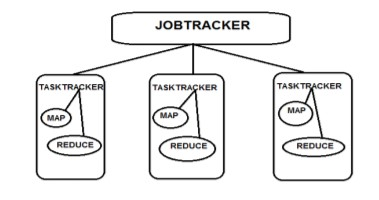
\includegraphics[scale=1]{mapreduce1}
	\caption{JobTracker dan TaskTracker}
	\label{fig:jobtracker}
\end{figure}

\noindent Pada Gambar \ref{fig:jobtracker}, pekerjaan pada MapReduce dikerjakan oleh dua elemen:

\begin{itemize}
\item JobTracker\\
JobTracker berjalan pada master node untuk memonitor tugas-tugas MapReduce yang telah dijalankan oleh TaskTracker pada node salve. Tugas JobTracker adalah mengalokasikan pekerjaan yang sesuai untuk TaskTracker tertentu tergantung pada berapa banyak slot tugas yang tersedia. TaskTracker mengatur pelaksanaan setiap operasi MapReduce pada setiap node slave. 
\item TaskTracker\\
TaskTracker berjalan pada masing-masing node slave. TaskTracker menerima pekerjaan dari JobTracker dan menjalankan operasi MapReduce. Setiap TaskTracker memiliki jumlah slot pekerjaan yang terbatas. Tugas masing-masing TaskTracker adalah memulai JVM untuk menjalankan operasi MapReduce secara paralel. 
\end{itemize}

\section{Spark} 
Spark adalah teknologi komputasi cluster kilat-cepat, yang dirancang untuk komputasi cepat. Spark adalah paradigma pemrosesan data berukuran besar yang dikembangkan oleh para peneliti University of California di Berkeley. Spark adalah alternatif untuk Hadoop yang dirancang untuk mengatasi keterbatasan pemrosesan input output pada disk dan meningkatkan kinerja sistem sebelumnya. Fitur utama Spark yang membuatnya unik adalah kemampuannya untuk tampil dalam perhitungan memori. Ini memungkinkan data di-cache dalam memori, sehingga menghilangkan overhead disk Hadoop keterbatasan untuk tugas berulang. 
 
\par Spark dirancang untuk mencakup pembagian beban kerja secara adil dalam sistem terdistribusi yang terpisah. Dengan memanfaatkan sistem terdistribusi yang ada, Spark menjadi alternatif untuk melakukan komputasi secara paralel dalam analisis data sehingga proses yang besar dapat dilakukan dengan mudah dan murah. Spark bertanggung jawab untuk melakukan penjadwalan, distribusi, dan memonitor jalannya komputasi pada banyak komputer. Spark adalah mesin umum untuk pemrosesan data skala besar yang mendukung Java, Scala dan Python dan untuk tugas-tugas tertentu diuji hingga 100 kali lebih cepat dari Hadoop MapReduce ketika data dapat muat dalam memori dan hingga 10 kali lebih cepat ketika data berada pada disk.

\subsection{Ekosistem Spark}
\begin{figure}[H]
	\centering
	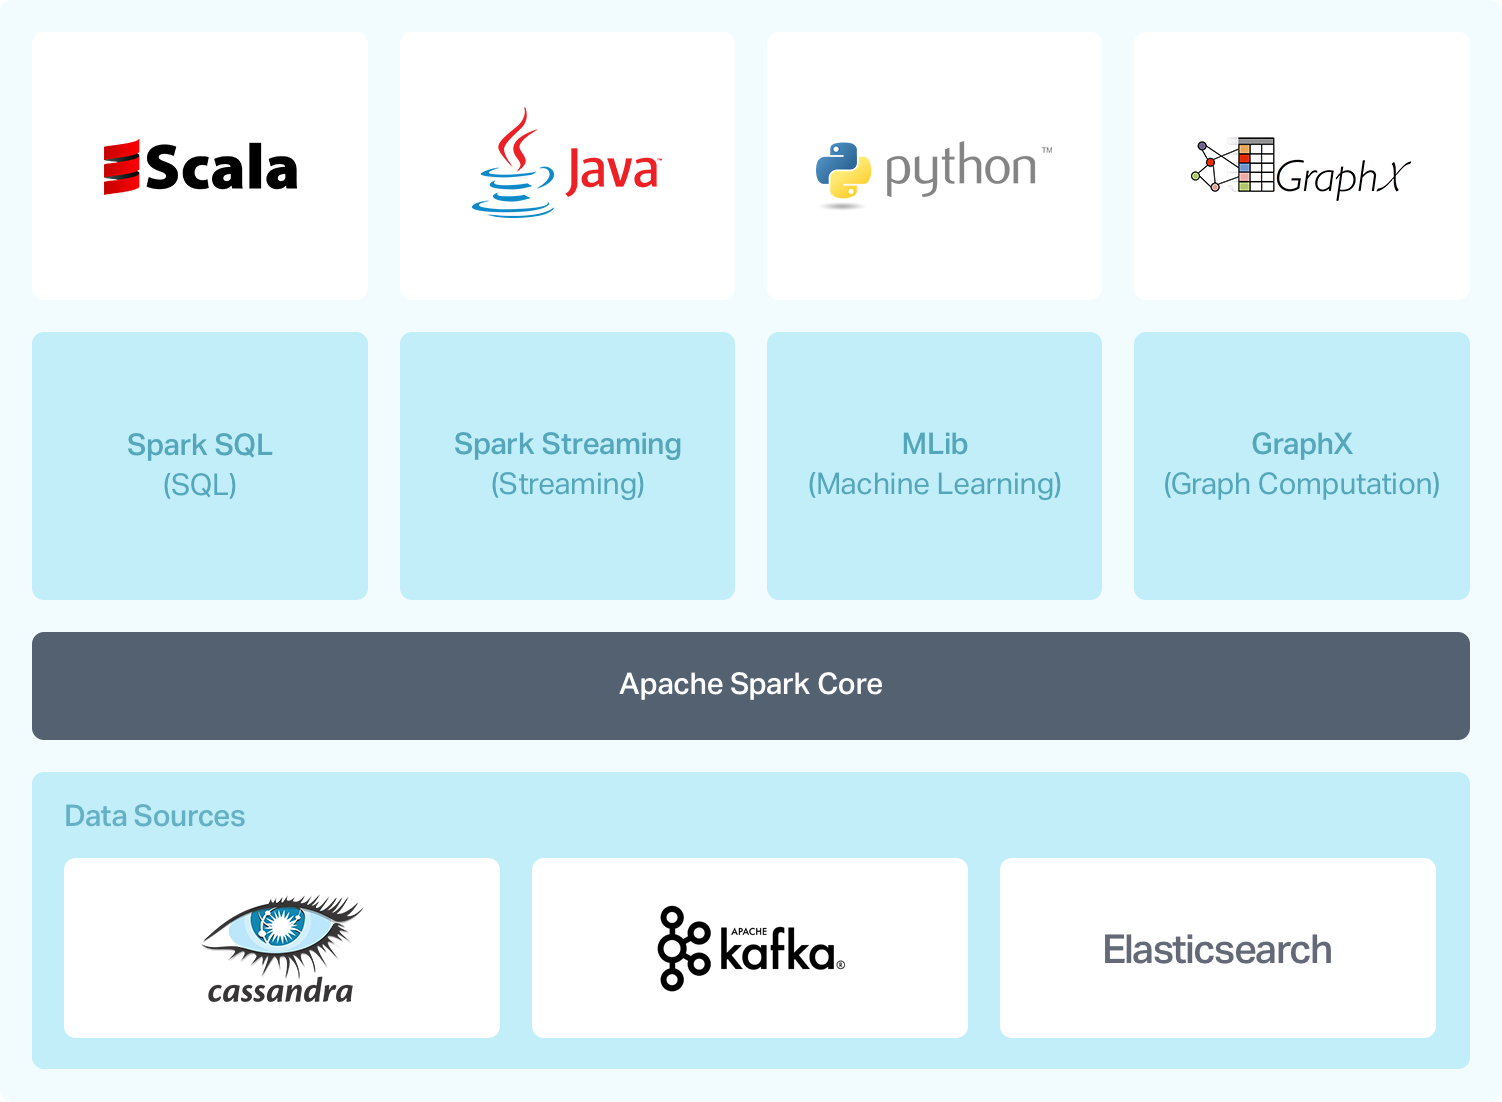
\includegraphics[scale=0.16]{spark_ecosystem}
	\caption{Ekosistem Spark}
	\label{fig:spark_ecosystem}
\end{figure}
Melalui Gambar \ref{fig:spark_ecosystem}, Spark bekerja sama dengan teknologi lain untuk memenuhi berbagai macam kebutuhan dalam pengolahan big data. Masing-masing warna pada Gambar \ref{fig:spark_ecosystem} mewakili jenis teknologi yang dipakai pada Spark. Spark SQL, Spark Streaming, Spark MLlib adalah library tambahan pada Spark. Cassandra, Kafka, dan ElasticSearch adalah framework untuk melakukan pengumpulan data secara streaming. Sedangkan scala, java, dan python adalah bahasa pemrograman yang dapat digunakan pada Spark.

\subsection{Arsitektur Spark}
\begin{figure}[H]
	\centering
	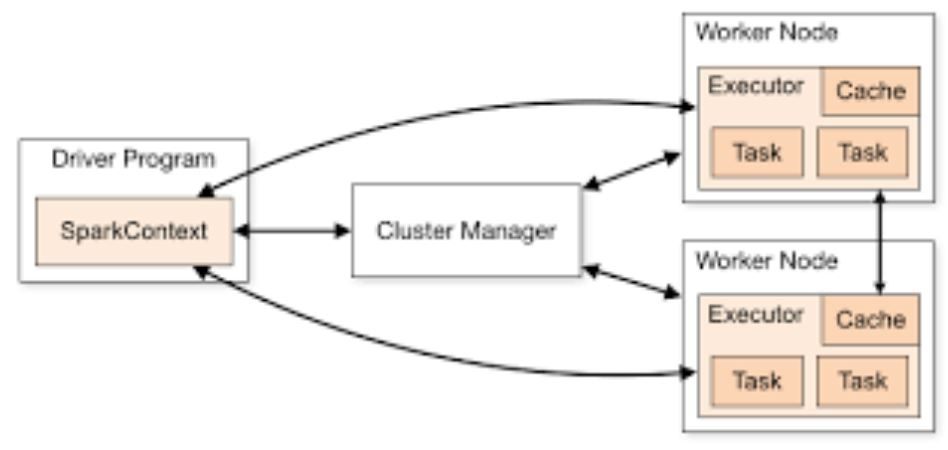
\includegraphics[scale=0.8]{arsitektur_spark2}
	\caption{Arsitektur Spark}
	\label{fig:arsitektur_spark2}
\end{figure}

\noindent Beberapa hal penting pada Gambar\ref{fig:arsitektur_spark2} terkait arsitektur Spark adalah sebagai berikut:

\begin{itemize}
\item Driver Program\\
Driver Program adalah komputer yang sedang menjalankan perintah-perintah pada Spark (perintah SparkContext). 
\item Cluster Manager\\
Cluster Manager disebut juga master node, bertugas untuk mengatur jumlah pekerjaan yang diberikan untuk masing node "worker" dan jumlah node "worker" yang diperlukan.
\item Worker Node\\
Worker Node adalah node yang akan mengerjakan seluruh tugas yang telah diberikan oleh cluster manager.
\end{itemize}


\subsection{Jenis Instalasi pada Spark}
\begin{figure}[H]
	\centering
	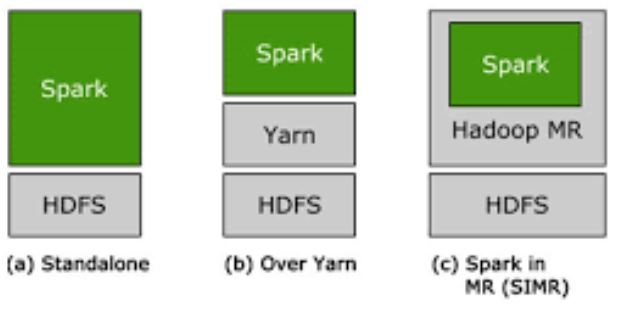
\includegraphics[scale=0.9]{arsitektur_spark}
	\caption{Arsitektur Spark}
	\label{fig:arsitektur_spark}
\end{figure}

Berdasarkan Gambar \ref{fig:arsitektur_spark}, berikut adalah tiga metode yang dapat dilakukan dalam  instalasi Spark:

\begin{itemize}
\item Standalone\\  
Spark berdiri diatas HDFS Hadoop. Pada metode instalasi ini, Spark dan Hadoop akan berjalan bersamaan pada mesin yang sama. Selain itu, Spark memungkinkan untuk mengakses data pada HDFS Hadoop untuk membaca input dan menulis output.

\item Hadoop Yarn adalah \\
Hadoop Yarn berarti Spark bekerja pada Yarn tanpa memerlukan instalasi atau meminta hak akses root apapun. Hadoop Yarn membantu untuk mengintegrasikan Spark pada ekosistem Hadoop dan memungkinkan komponen lain berjalan di atas Spark.

\item Spark In MapReduce (SIMR)\\ 
SIMR digunakan untuk menjalankan pekerjaan Spark secara independen. Pada metode instalasi ini, pengguna dapat memulai Spark menggunakan perintah "spark-shell" tanpa perlu ijin dari administrator. Pada versi Spark 2.0 keatas, metode instalasi ini sudah tidak dapat lagi dipakai.
\end{itemize}

\subsection{RDD pada Spark}
\par Spark menawarkan abstraksi Resilient distributed Datasets (RDD) untuk mendukung pemrosesan data secara efisien. RDD adalah kumpulan data yang didistribusikan. Dalam Spark semua pekerjaan dinyatakan dengan membuat RDD baru, mengubah RDD yang ada, atau memanggil operasi pada RDD untuk menghitung hasilnya. RDD mendukung dua jenis operasi yaitu transformation dan action. Spark secara otomatis mendistribusikan data dalam RDD di seluruh cluster komputasi dan melakukan komputasi secara paralel. RDD dapat disimpan dalam memori antara banyak kueri tanpa membutuhkan replikasi. RDD dapat membangun kembali data yang hilang pada kegagalan menggunakan riwayat pembentukan setiap RDD mengingat RDD dibangun dari kumpulan data lain (melalui fungsi transformasi seperti map, join, dan group By). RDD memungkinkan Spark untuk mengungguli model yang ada hingga 100x dalam menganalisis data. RDD dapat mendukung berbagai macam algoritma machine learning untuk melakukan teknik data mining secara interaktif dan menyediakan pemrograman SQL yang sangat efisien.

\newpage
\noindent Berikut adalah penjelasan singkat dan contoh dari jenis operasi pada RDD:

\begin{itemize}
\item Transformation\\
Tranformation adalah operasi pada RDD untuk mengembalikan output berupa RDD baru. Transformatsi pada RDD dilakukan secara lazy, sehingga tranformasti hanya akan dikerjakan apabila dipanggil pada sebuah action. Contoh dari transformasi adalah map(), flatmap(), filter(), groupByKey(), lessByKey(), mapValues().

\item Action\\
Action adalah operasi yang mengembalikan nilai output ke dalam terminal atau melakukan penulisan data pada sistem penyimpanan eksternal. Action memaksa evaluasi pada RDD yang akan dipanggil, untuk menghasilkan output. Contoh dari action adalah take(), count(), collect(), reduce(), takeOrdered(), top().
\end{itemize}
 
 

\subsection{Komponen Spark}
Komponen Spark adalah library tambahan pada Spark untuk melakukan proses komputasi pada lingkungan big data berdasarkan jenis-jenis kebutuhan pengolahan data. Pada umumnya, Spark hanya membutuhkan library Spark Core saja untuk melakukan komputasi sederhana seperti pemrosesan pada MapReduce. Untuk kasus-kasus tambahan seperti implementasi kueri SQL dan teknik data mining digunakan library tambahan yaitu Spark Core dan Spark SQL. 
\\\\
Berikut adalah penjelasan singkat mengenai jenis library pada Spark:

\begin{itemize}
\item Spark Core \\
Spark Core adalah library Spark yang berisi fungsionalitas dasar Spark, termasuk komponen untuk penjadwalan tugas, manajemen memori, pemulihan kesalahan, dan berinteraksi dengan sistem penyimpanan. Spark Core juga merupakan rumah bagi API yang mendefinisikan set data terdistribusi yaitu (RDD), yang merupakan abstraksi pemrograman utama Spark. RDD merupakan kumpulan item yang didistribusikan di banyak node komputasi yang dapat dimanipulasi secara paralel.
\item Spark SQL  \\
Spark SQL adalah library Spark untuk bekerja dengan data terstruktur. Spark SQL memungkinkan pemrosesan kueri SQL pada lingkungan big data. Selain itu, Spark SQL menyediakan antarmuka SQL untuk Spark. Hasil pemrosesan kueri pada Spark SQL dapat digabungkan dengan hasil manipulasi data oleh RDD, sehingga memungkinkan untuk melakukan analisis data dengan lebih variatif.
\item
Spark MLlib \\
Spark MLlib adalah library Spark yang berisi fungsionalitas yang umum digunakan pada Machine Learning (ML). Untuk mengimplementasikan teknik data mining pada lingkungan big data dibutuhkan library Spark MLlib. Spark MLlib menyediakan berbagai jenis algoritma Machine Learning termasuk klasifikasi, regresi, pengelompokan/clustering, dan filter kolaboratif, dan fungsionalitas pendukung seperti evaluasi model dan impor data. Semua metode pada Spark MLlib ini dirancang untuk pemrosesan Machine Learning pada lingkungan big data.
\end{itemize}

\newpage
\subsection{Perbandingan Hadoop dan Spark}

Berikut ini adalah studi perbandingan analisis data menggunakan Hadoop dan Spark:
\\\\
\begin{tabular}{|p{7.5cm}|p{7.5cm}|}
\hline 
Hadoop & Spark \\ 
\hline 
Hadoop tidak efisien untuk pengolahan data dengan berbagi data ke setiap kluster, karena memiliki latensi rendah. & Spark memungkinkan melakukan steream processing pada data yang besar  dengan memotong-motong data menjadi ukuran yang lebih kecil yang dapat ditampung oleh memori \\ 
\hline 
Lebih lambat karena hasil pengolahan data disimpan di
hard disk. & Memiliki kecepatan 100 kali lebih cepat dibandingkan Hadoop, karena hasil pemrosesan data disimpan dalam memori. \\ 
\hline 
Kompatibel melakukan stream processing, machine learning, dan kueri basisdata. & Kompatibel terhadap Spark streaming, Spark MLLib untuk machine learning,  dan Spark SQL untuk melakukan kueri pada data terstruktur. \\ 
\hline 
Pemakaian memori yang lebih rendah. & Pemakaian memori lebih tinggi. Dapat melakukan degradasi dalam
membagi pekerjaan apabila data tidak muat di memori. \\ 
\hline 
Output disimpan dalam disk. & Sistem operasi akan memutuskan apakah output data akan disimpan dalam memori atau disimpan dalam hard disk. \\ 
\hline 
\end{tabular} 



\section{Scala}
Scala adalah bahasa pemrograman berbasi open source, dibuat oleh Profesor Martin Odersky. Scala adalah bahasa pemrograman multi-paradigma dan mendukung paradigma fungsional serta berorientasi objek. Apache Spark ditulis dalam Scala dan karena skalabilitasnya di JVM. Pemrograman scala adalah bahasa pemrograman yang paling banyak digunakan, oleh pengembang big data untuk mengerjakan proyek Spark.

\par Scala digunakan untuk mengakses dan mengimplementasikan fitur-fitur Spark dengan mudah. Kesamaan antara Scala dengan Java adalah memakai konsep object oriented dengan bahasa pemrograman yang lebih disederhanakan. Scala menyediakan jalur terbaik untuk membangun aplikasi big data untuk menangani permasalahan pada kompleksitas program. Scala mendukung konsep parallel dan concurrency untuk pemodelan MapReduce dan sangat cocok untuk implementasi pada pemrograman fungsional. Scala memiliki kelebihan pada concurrency dan library bawaan yang sangat beragam. 

\par Untuk pengembangan Spark, penulisan sintaks Scala dianggap produktif untuk mengimplementasikan kode program. Pemrograman pada Scala mempertahankan prinsip keseimbangan antara produktivitas pengembangan program dan kinerja program. Pemrograman pada Scala tidak serumit pemrograman pada Java. Satu baris kode program pada Scala dapat menggantikan 20 hingga 25 baris kode java. Karena alasan terbut, Scala menjadi bahasa pemrograman yang sangat diminati untuk melakukan pemrosesan big data pada Apache Spark.


\section{Scala Swing} 
Scala swing mengimplementasikan program dengan Graphical User Interface (GUI), berbeda dengan program Spark pada umumnya yang hanya melakukan eksekusi dengan menggunakan terminal. Penggunaan terminal terbatas pada penerimaan input dan penampilan output. Dengan menggunakan program berbasis GUI, diharapkan interaksi pada program menjadi lebih beragam. Perbedaan utama antara terminal dan GUI adalah program berbasis terminal menjalankan prosedur yang tetap, sedangkan program berbasis GUI menjalankan prosedur sesuai dengan kebutuhan penggunanya.

\par Scala menyediakan akses langsung terhadap kelas GUI Java menggunakan library Scala Swing. Secara konseptual, library Scala Swing menyerupai library Java Swing pada Java. Akan tetapi, Scala Swing lebih menyembunyikan kerumitan kode dibandingkan library Java Swing. Dengan menggunakan Scala, penggunaan library Scala Swing memenuhi kebutuhan perancangan User Interface, dengan tersedianya berbagai macam fitur GUI pada umumnya.

\par Dasar untuk menyusun aplikasi GUI adalah membangun komponen GUI.  Library Scala Swing menyediakan komponen Frame, Panel, Label dan Button yang sama seperti komponen GUI pada umumnya. Komponen pada Scala Swing memiliki properti yang dapat diatur secara manual. Beberapa komponen pada Scala Swing dapat menangani handling event tertentu. Handling event adalah perkerjaan yang dilakukan sebuah komponen, ketika komponen tersebut menerima aksi secara langsung dari pengguna aplikasi.

\section{Jenis Data Input}
Spark menerima berbagai jenis data input dan menfasilitasi penulisan berbagai jenis data output, karena Spark dibangun di atas ekosistem Hadoop. Secara khusus, Spark dapat mengakses data melalui antarmuka format input dan output yang digunakan oleh Hadoop Map Reduce. Berberapa jenis data yang akan diolah memiliki format penulisan masing-masing, sehingga memiliki cara yang berbeda untuk mengambil sekumpulan data dalam format tersebut. Berikut adalah contoh format data yang akan digunakan pada proses pengolahan data.   

\subsection{CSV}
Comma Separated Value (CSV) berisi sejumlah jumlah atribut data untuk setiap baris dan dipisahkan oleh koma. CSV tidak memiliki format yang konsisten. Beberapa hal yang sering terjadi terkait penulisan format yang salah pada CSV adalah penggunaan karakter non-ASCII. CSV tidak dapat mengakses nilai atribut data secara langsung. Untuk mendapatkan nilai atribut secara spesifik, perlu dilakukan pemisahan koma untuk setiap baris data. Dalam beberapa tahun terakhir, penggunaan struktur CSV untuk penyimpanan data semakin meningkat. Semakin banyaknya kebutuhan pengolahan data berdasarkan format CSV, maka perlu mencari tahu teknik penyimpanan dan pengambilan data CSV pada Spark. Spark mampu melakukan proses manipulasi dan transformasi data CSV tanpa menggunakan library tambahan.

\subsection{XML}
XML menyediakan format penulisan data menggunakan tag pembuka dan penutup. Tag pembuka dan penutup pada XML ditulis dengan tujuan memberi tahu data-data apa saja yang merupakan cakupan dari elemen tag tersebut. Dalam beberapa tahun terakhir, pengolahan data dengan format XML semakin meningkat seiring berkembangnya pemakaian XML sebagai format penyimpanan data.  Oleh karena itu, perlu adanya cara untuk menyimpan dan mengambil nilai sebuah data pada file yang beformat XML. Berkembangan format penyimpanan XML menghadirkan tantangan baru bagi pengolahan big data, karena Spark tidak mampu melakukan proses manipulasi dan transformasi data XML tanpa menggunakan  library tambahan.
